\documentclass[12pt]{extarticle}
\usepackage{geometry}
\geometry{
a4paper,
total={170mm,257mm},
left=20mm,
top=20mm,
headheight=12pt
}
\usepackage[parfill]{parskip} % Activate to begin paragraphs with an empty line rather than an indent
\usepackage{graphicx} % Use pdf, png, jpg, or eps§ with pdflatex; use eps in DVI mode
% TeX will automatically convert eps --> pdf in pdflatex		

\usepackage{amssymb,amsmath,amsthm}
\usepackage{commath}
\usepackage{longtable}
\usepackage[hyphens]{url}
\usepackage[dvipsnames]{xcolor}
\usepackage[unicode=true,colorlinks=true,urlcolor=CadetBlue,citecolor=black,linkcolor=black]{hyperref}
\PassOptionsToPackage{hyphens}{url} % url is loaded by hyperref
\usepackage{authblk}
\usepackage{subcaption}
\captionsetup[subfigure]{labelformat=empty}
\usepackage[font=small,labelfont=bf]{caption}
\usepackage{longtable}
\usepackage{gensymb,siunitx}

%SetFonts
% newtxtext+newtxmath
\usepackage{newtxtext} %loads helv for ss, txtt for tt
\usepackage{amsmath}
\usepackage[bigdelims]{newtxmath}
\usepackage[T1]{fontenc}
\usepackage{textcomp}
%SetFonts

\renewcommand{\baselinestretch}{1.5}

% less space before sections 
% \@startsection {NAME}{LEVEL}{INDENT}{BEFORESKIP}{AFTERSKIP}{STYLE} 
%            optional * [ALTHEADING]{HEADING} 
\makeatletter
 \renewcommand\section{\@startsection {section}{1}{\z@}%
     {-2.5ex \@plus -1ex \@minus -.2ex}%
     {1.3ex \@plus.2ex}%
    {\Large\bfseries}}
    
% Species names
%% Meta-Command for defining new species macros
\usepackage{xspace}

\newcommand{\species}[3]{%
  \newcommand{#1}{\gdef#1{\textit{#3}\xspace}\textit{#2}\xspace}}
  
\species{\yeast}{Saccharomyces cerevisiae}{S.~cerevisiae}
\species{\calbicans}{Candida albicans}{C.~albicans}
\species{\cneoformans}{Cryptococcus neoformans}{C.~neoformans}

% Yoav & Lee commands
\newcommand*{\tr}{^\intercal}
\let\vec\mathbf
\newcommand{\matrx}[1]{{\left[ \stackrel{}{#1}\right]}}
\newcommand{\diag}[1]{\mbox{diag}\matrx{#1}}
\newcommand{\goesto}{\rightarrow}
\newcommand{\dspfrac}[2]{\frac{\displaystyle #1}{\displaystyle #2} }
\newtheorem{theorem}{Theorem}
\newtheorem{corollary}{Corollary}
\newtheorem{lemma}{Lemma}
\newtheorem{remark}{Remark}
\newtheorem{result}{Result}
\renewcommand\qedsymbol{} % no square at end of proof
\newcommand{\cl}{\mathbf{L}}
\newcommand{\cj}{\mathbf{J}}
\newcommand{\ci}{I}
\newcommand{\likelihood}{\mathcal{L}}

% genotype commands
\newcommand{\euwt}{\emph{2n}}
\newcommand{\anwt}{\emph{2n+1}}
\newcommand{\eumt}{\emph{2n*}}
\newcommand{\anmt}{\emph{2n+1*}}

% Supplementary
\newcommand{\beginsupplement}{%
      	\setcounter{table}{0}
        \renewcommand{\thetable}{S\arabic{table}}%
        \setcounter{figure}{0}
        \renewcommand{\thefigure}{S\arabic{figure}}%
}

% NatBib
\usepackage[round,colon,authoryear]{natbib}

% Title page
% Chromosomal duplication is a transient evolutionary solution to stress
%\title{Clonal interference between aneuploidy and mutation}
\title{Adaptive evolution with aneuploidy and mutation}

% Authors
\renewcommand\Affilfont{\small}

\author[1,*]{Ilia Kohanovski}
\author[2,*]{Martin Pontz}
\author[3]{Avihu H. Yona}
%\author[d]{Orna Dahan}
%\author[d]{Yitzhak Pilpel}
\author[1,2,$\dagger$]{Yoav Ram}

\affil[1]{School of Computer Science, Reichman University, Herzliya, Israel}
\affil[2]{School of Zoology, Faculty of Life Sciences, Tel Aviv University, Tel Aviv, Israel}
\affil[3]{Institute of Biochemistry, Food Science and Nutrition,
Robert H. Smith Faculty of Agriculture, Food and Environment,
The Hebrew University of Jerusalem, Israel}
%\affil[d]{Department of Molecular Genetics, Weizmann Institute of Science, Rehovot 76100, Israel}
\affil[*]{These authors contributed equally to this work}
\affil[$\dagger$]{Corresponding author: yoav@yoavram.com}

% Document
\begin{document}
\maketitle

% Abstract
\begin{abstract}
Aneuploidy is common in eukaryotes, often leading to decreased cell growth and fitness. However, evidence from yeast and fungi, as well as human tumour cells, suggests that aneuploidy can be beneficial under stressful conditions and lead to elevated growth rates and adaptation.
Importantly, aneuploidy differs from point mutations in rate, fitness effect, and reversibility.
Here, we develop evolutionary models for adaptive evolution with both mutation and aneuploidy. 
These models are used within an approximate Bayesian computation framework to estimate the formation rate and fitness effect of aneuploidy and mutation from  results of evolutionary experiments in which \yeast adapted to heat stress: the experimental populations first acquired chromosome duplications, only to later revert back to a euploid state.
We also analyze our models to estimate the effect of the aneuploidy and mutation rates on the expected adaptation time and the probability for adaptation via aneuploidy.
Our results suggest that aneuploidy can be a transient adaptive solution, which can decelerate adaptation in a non-intuitive manner. By creating an evolutionary conflict between the individual and the population, aneuploidy further complicates the process of adaptation in cell populations.
\end{abstract}

% TODO cite https://www.biorxiv.org/content/10.1101/2020.10.07.327759v1
% TODO cite Yang, F. et al. The fitness costs and benefits of trisomy of each Candida albicans chromosome. Genetics 218, 1–7 (2021). https://academic.oup.com/genetics/article/218/2/iyab056/6218773
% cite: https://www.cell.com/developmental-cell/fulltext/S1534-5807(21)00562-1?_returnURL=https%3A%2F%2Flinkinghub.elsevier.com%2Fretrieve%2Fpii%2FS1534580721005621%3Fshowall%3Dtrue
% cite: https://www.cell.com/developmental-cell/fulltext/S1534-5807(21)00592-X?_returnURL=https%3A%2F%2Flinkinghub.elsevier.com%2Fretrieve%2Fpii%2FS153458072100592X%3Fshowall%3Dtrue

\pagebreak
% Introduction
\section*{Introduction}

\paragraph*{Aneuploidy is common in eukaryotes.}
Aneuploidy is an imbalance in the number of chromosomes in the cell: an incorrect karyotype.
Evidence suggests aneuploidy is very common in eukaryotes, e.g. animals~\citep{Santaguida2015review, Naylor2016, Bakhoum2017}, and fungi~\citep{Pavelka2010, Zhu2016, Robbins2017, Todd2017}.
Aneuploidy has been implicated in cancer formation and progression~\citep{Boveri2008, Schvartzman2010}: 
90\% of solid tumours and 50\% of blood cancers are aneuploid~\citep{Santaguida2015review}.
Aneuploidy is also linked to the emergence of drug resistance~\citep{Selmecki2009} and virulence~\citep{Moller2018} in fungal pathogens, which are under-studied~\citep{Rodrigues2018} despite infecting close to a billion people per year, causing serious infections and significant morbidity in >150 million people per year and killing >1.5 million people per year~\citep{Selmecki2009, Rodrigues2018}.
In addition, aneuploidy is common in protozoan pathogens of the Leishmania genus, a major global health concern~\citep{Mannaert2012}.

\paragraph*{Aneuploidy is generally deleterious.}
The molecular and genetic mechanisms involved in aneuploidy have been explored~\citep{Musacchio2007, Sheltzer2011, Chen2012b, Rancati2013, Gerstein2015, Shor2015}.
Experiments with human and mouse embryos found that aneuploidy is usually lethal.
It is also associated with developmental defects and lethality in other multicellular organisms~\citep{Sheltzer2011}. For example, aneuploid mouse embryonic cells grow slower than euploid cells~\citep{Williams2008}.
Similarly, in unicellular eukaryotes growing in benign conditions, aneuploidy usually leads to slower growth and decreased overall fitness~\citep{Niwa2006, Torres2007, Pavelka2010, Sheltzer2011, Kasuga2016}, in part due to proteotoxic stress caused by increased expression in aneuploid cells~\citep{Pavelka2010, Santaguida2015, Zhu2018} and hypo-osmotic-like stress~\citep{Tsai2019}.

\paragraph*{Aneuploidy can lead to adaptation.}
However, aneuploidy can be beneficial under stressful conditions due to the wide range of phenotypes it can produce, some of which are advantageous~\citep{Pavelka2010}.
Thus, aneuploidy can lead to rapid adaptation in unicellular eukaryotes~\citep{Gerstein2015,Torres2010, Hong2014, Rancati2008}, as well as to rapid growth of somatic tumour cells~\citep{Schvartzman2010, Sheltzer2017}.
For example, aneuploidy in \yeast facilitates adaptation to a variety of stressful conditions like heat and pH~\citep{Yona2012}, copper~\citep{Covo2014, Gerstein2015}, salt~\citep{Dhar2011}, and nutrient limitation~\citep{Dunham2002, Gresham2008}.
Importantly, aneuploidy can also lead to drug resistance in pathogenic fungi such as \calbicans~\citep{Selmecki2008, Selmecki2010, Gerstein2018} and \cneoformans~\citep{Sionov2010}, which cause candidiasis and meningoencephalitis, respectively.

\paragraph*{Transient adaptive solution.} 
Aneuploidy differs from mutation due to its distinct properties. 
Chromosome duplication usually occurs more often than mutation and on average produces larger fitness effects.
Yet, because it affects many genes on a whole chromosome or a chromosome fragment, aneuploidy also carries fitness costs.
Thus, aneuploidy can be a \emph{transient adaptive solution}: it can rapidly occur and fix in the population under stressful conditions, and can be rapidly lost when the cost outweighs the benefit---when stress is removed or after beneficial mutations occur.
Experimental evidence of such a transient role of aneuploidy was demonstrated by \citet{Yona2012}. They evolved populations of \yeast under strong heat or pH stress.
The populations adapted to the heat and pH stress within 450 and 150 generations, and this adaptation was determined to be due to chromosome duplications.
Much later, after more than 1500 and 750 generations, for the heat and pH stress, respectively, the populations reverted back to an euploid state, while remaining adapted to the stress and accumulating multiple mutations.
However, under gradual heat stress, aneuploidy was not observed.
\citet{Yona2012} concluded that aneuploidy serves as a transient adaptive solution, or a ``quick fix'', which is expected to facilitate adaptation. 

\paragraph*{The present study.}
Here, we develop evolutionary-genetic models that include the effects of natural selection, genetic drift, aneuploidy, and mutation to examine the role of aneuploidy in adaptive evolution.
These models follow a population of cells characterised by both their ploidy and their genotype.
We fit these models to the experimental results of \citet{Yona2012} using an \emph{approximate Bayesian computation} framework~\citep{Sisson2009} to infer model parameters, including selection coefficients and rates of aneuploidy and mutation, and to perform model selection between different models, thereby testing hypotheses about the evolutionary process. 
We analyze these evolutionary-genetic models to estimate the effects of parameters on the adaptation time and the probability for adaptation via aneuploidy.
We find that \textbf{TODO} % TODO 

\pagebreak
%%%%%%%%%%%%%%%%%%%%%%%%
% Models and Methods
\section*{Models and Methods}

%%%%%%%% Fig illustation
\begin{figure}[b!]
  %\centering
  \begin{subfigure}[t]{0.4\textwidth}
      \caption{
        \textbf{A. Single-locus model}
      }
      \centering
      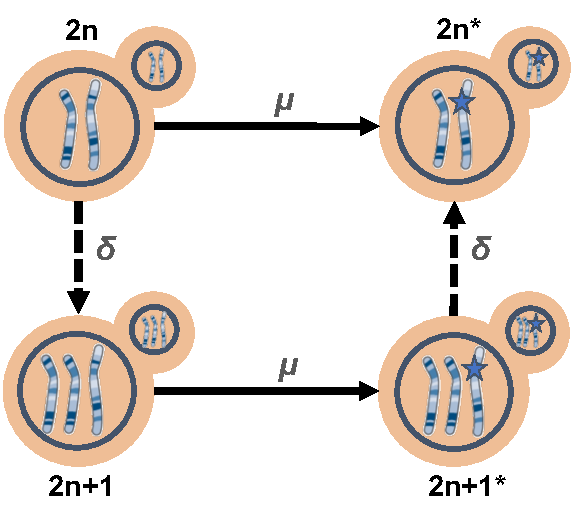
\includegraphics[height=1.8in]{../figures/Fig1-A.pdf}      
      \label{fig:model1}
  \end{subfigure}
  %\\
  \begin{subfigure}[t]{0.4\textwidth}
  	  \caption{
        \textbf{B. Multi-locus model}
      }
      \centering
      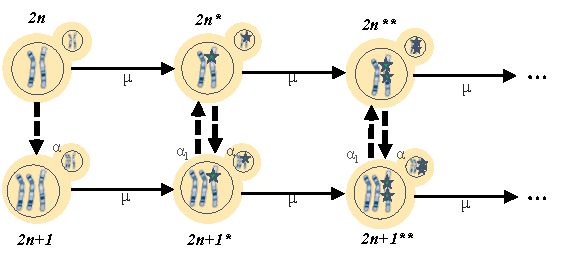
\includegraphics[height=1.8in]{../figures/Fig1-B.pdf}      
      \label{fig:model2}
  \end{subfigure}
  \caption{
    \textbf{Model illustrations.}
    \textbf{(A)} In the single-locus model, the four genotypes are: euploid wild-type, \euwt; euploid mutant, \eumt; aneuploid wild-type, \anwt; and aneuploid mutant, \anmt.
    Overall there are two possible trajectories from \euwt\; to \eumt.
    \textbf{(B)} In the multi-locus model, each genotype is characterized by its karyotype, \euwt\; or \anwt, and the number of accumulated beneficial mutations, denoted by stars. 
    In both panels arrows denote transitions between genotypes, with transitions rates: $\mu$, beneficial mutation rate; $\delta$, aneuploidy rate.
  }
  \label{fig:models}
\end{figure}
%%%%%%%%%%%%%%%%%%%%%%%%

%%%%%%%%%%%%%%%%%%%%%%%%
\paragraph*{Evolutionary Models.}
We model the evolution of a population of cells using two models: a single-locus model and a multi-locus model.
Both models are based on the Wright-Fisher model~\citep{Otto2007}, assuming non-overlapping generations and including the effects of natural selection, genetic drift, aneuploidy, and mutation. 
We focus on beneficial mutations, neglecting the effects of deleterious and neutral mutations. Both models allow for a single aneuploid karyotype (e.g., chromosome III duplication).
While the single-locus model allows for only a single mutation to accumulate in the genotype, the multi-locus model allows for multiple mutations to accumulate~(\autoref{fig:models}), as well as for a fluctuating population size.

%%%%%%%%%%%%%%%%%%%%%%%%
\paragraph*{Single-locus model.}
This model assumes a constant effective population size $N$ and follows four genotypes~(\autoref{fig:models}A): euploid wild-type, \euwt, the initial genotype; 
euploid mutant, \eumt, with the standard karyotype and a single beneficial mutation; 
aneuploid wild-type, \anwt, with an extra chromosome, i.e., following chromosome duplication; and
aneuploid mutant, \anmt, with and extra chromosome and a beneficial mutation. 

Transitions between the genotypes occur as follows~(\autoref{fig:models}A): Beneficial mutations from \euwt\; to \eumt\; and from \anwt\; to \anmt\; occur with probability $\mu$, the mutation rate. We neglect back-mutations (i.e., from \eumt\; to \euwt\; and from \anmt\; to \anwt).
Aneuploidy is formed by chromosome mis-segregation, so that cells transition from \euwt\; to \anwt\; and from \anmt\ to \eumt\ with probability $\delta$, the aneuploidy rate. That is, we assume chromosomes are gained and lost at the same rate, and we neglect events that form a less-fit genotype (i.e., \anwt\; to \euwt\; and \eumt\; to \anmt).
The fitness values of the four genotypes are given by \autoref{table:single-locus}.

%%% Table: single-locus model
\begin{table}[h]
\centering
\caption{\textbf{Single-locus model fitness values.}}
\begin{tabular}{lllll}
\emph{Genotype} $i$ & $2n$ & $2n+1$ & $2n+1^*$ & $2n^*$ \\
\hline
\emph{Fitness} $w_i$ & $1$ & $1-c+b$ & $(1-c)(1+s)+b$ & $1+s$               
\end{tabular}
\label{table:single-locus}
\caption*{
$s \ge 0$ is the selection coefficient of a beneficial mutation;
$0 \le c \le 1$ is the fitness cost of aneuploidy;
and $b \ge c$ is the selection coefficient, or fitness benefit, of aneuploidy.
}
\end{table}
%%%%%%%%%%%%%%%%%%%%%%%%

The initial population has $N$ cells with genotype \euwt.
The effect of natural selection on the frequency $f_i$ of genotype $i = 2n, 2n+1, 2n+1^*, \text{or } 2n^*$ is given by
    \begin{equation} \label{eq:selection-single} 
      f^s_i = \frac{f_i w_i}{\bar{w}} \;,
    \end{equation}
where the fitness values $w_i$ are given in \autoref{table:single-locus} and $\bar{w} = \sum_{j}{f_j w_j}$ is the population mean fitness.
The effect of mutation and aneuploidy on genotype frequencies is given by
    \begin{equation} \label{eq:mutation-aneuploidy-single}
    \begin{aligned}
      &f^m_{2n} &=&\; (1 - \delta - \mu) f^s_{2n}  \;,\\
      &f^m_{2n+1} &=&\; \delta f^s_{2n} + (1 - \mu) f^s_{2n+1}  \;,\\
      &f^m_{2n+1^*} &=&\; \mu f^s_{2n+1} + (1-\delta) f^s_{2n+1^*}  \;,\\
      &f^m_{2n^*} &=&\; \mu f^s_{2n} + \delta f^s_{2n+1} + f^s_{2n^*}  \;.
    \end{aligned}
    \end{equation}
Finally, random genetic drift is modeled using a multinomial distribution~\citep{Otto2007},
    \begin{equation} \label{eq:drift-single}
      \vec{f'} \sim \frac{1}{N} \cdot \mathit{Mult}(N,\ \vec{f^m}) \;,
    \end{equation}
where $\vec{f^m}=(f^m_{2n}\ ,\ f^m_{2n+1}\ ,\ f^m_{2n+1^*}\ ,\ f^m_{2n^*})$ are the frequencies of the genotypes after mutation and aneuploidy, $\vec{f'}$ are the genotype frequencies in the next generation, and $Mult(N,\ \vec{f})$ is a multinomial distribution parameterized by the population size $N$ and the genotype frequencies $\vec{f}$.
Overall, the change in genotype frequencies from one generation to the next is given by the transformation $f_i \to f'_i$.

%%%%%%%%%%%%%%%%%%%%%%%%
\paragraph*{Multi-locus model.}
This model expands the single-locus model by allowing for (i) the accumulation of beneficial mutations, and (ii) a fluctuating population size. 

A genotype is characterized by its karyotype, \euwt\; or \anwt, and the number of accumulated beneficial mutations, which can be zero or more.
The selection coefficient of the $i$-th accumulated mutation in each individual, $s_i$, is drawn from an exponential distribution with expected value $s$: $s_i \sim \mathit{Exp{(s)}}$.
The rest of the parameters ($N$, $\mu$, $\delta$, $b$, $c$) are the same as in the single-locus model. However, since the multi-locus model allows several mutations with smaller fitness effects to accumulate, we expect the mutation rate to be higher compared to the single-locus model, which focuses on a single, large-effect mutation.

The fitness of the different genotypes is the same as in the single-locus model (\autoref{table:single-locus}), except that the fitness contribution of $k$ beneficial mutations is the product of their independent effects, $\prod_{i=1}^k(1+s_i)$, instead of the contribution of the single mutation allowed in the single-locus model, $(1+s)$, see \autoref{table:multi-locus}.
Therefore, aneuploidy loss would be favored by selection only if there are enough beneficial mutations and/or the selection coefficients $s_i$ are large enough. The intuition is that when the benefit of the accumulated beneficial mutations is small, ten the benefit of aneuploidy has a large effect; when the benefit of the accumulated beneficial mutations is large, then aneuploidy is no longer beneficial due of its fitness cost.

In contrast to the single-locus model, in the multi-locus model the population size fluctuates to model serial-transfer experimental protocol~\citep{Yona2012}: the population is serially diluted by transferring a fraction of the population (1/120) to a fresh medium approximately every seven generations. 
Thus, the population initial size is $N_0 = N$, and the population size is doubled every generation, $N_1=2N, N_2=4N, \ldots$, and diluted back to $N$ after seven generations such that $N_8=N$.

The change in frequencies due to selection is exactly the same as in the single-locus model (\autoref{eq:selection-single}), only applied using the fitness values in \autoref{table:multi-locus}. The change due to random genetic drift is also the same as in \autoref{eq:drift-single}, except that the frequencies vector is $\vec{f}=(f_{2n}\ ,\ f_{2n+1}\ ,\ f_{2n^*}\ ,\ f_{2n+1^*}\ ,\ f_{2n^{**}}\ ,\ f_{2n+1^{**}}\ ,\ \ldots)$ and that the population size changes between generations, as described above.

The effects of mutation and aneuploidy on genotype frequencies is more elaborate than in the single-locus model.
Genotype $i$ is classified according to its karyotype (\euwt\ or \anwt), the number of accumulated beneficial mutations ($k \ge 0$), and their fitness ($w_i$).
Each offspring cell inherits these properties from its mother cell.
Then, a new beneficial mutation is accumulated with probability $\mu$, such that the number of mutations is $k+1$, and its effect $s_{k+1}$ is drawn from an exponential distribution with expected value $s$, such that the contribution of the mutations to the fitness is $\prod_{j=0}^{k+1}{(1+s_j)}$.
Next, euploid offspring become aneuploid with probability $\delta$, and aneuploid offspring become euploid with probability $\delta_L$.

%%% Table: multi-locus model
\begin{table}[h]
\centering
\caption{\textbf{Multi-locus model fitness values.}}
\begin{tabular}{lllll}
\emph{Genotype}, $g$ & $2n$ & $2n+1$ & $2n+1^{*k}$ & $2n^{*k}$ \\
\hline
\emph{Fitness}, $w_g$ & $1$ & $1-c+b$ & $(1-c)\prod_{j=1}^k(1+s_i)+b$ & $\prod_{j=1}^k(1+s_i)$               
\end{tabular}
\label{table:multi-locus}
\caption*{
$k$ is the number of accumulated beneficial mutations;
$s \ge 0$ is the selection coefficient of a beneficial mutation;
$0 \le c \le 1$ is the fitness cost of aneuploidy;
and $b \ge c$ is the selection coefficient, or fitness benefit, of aneuploidy.
}
\end{table}
%%%%%%%%%%%%%%%%%%%%%%%%%%%

\paragraph{Empirical evidence.}

We use the results of evolutionary experiments reported by \citet{Yona2012}.
In their heat-stress experiment, four populations of \yeast evolved under \SI{39}{\celsius}. Aneuploidy fixed in all four population in the first 450 generations (hereafter, fixation or elimination of a genotype \emph{by generation $t$} means that more than 95\% or less than 5\% of the population carry the genotype at generation $t$, and possibly earlier). From unpublished results, aneuploidy did not fix before at least 200 generations elapsed.
The experiment continued with two populations, in which aneuploidy was eliminated by generation 1,700 and 2,350.


\paragraph{Likelihood function.} 
Because our model, just like the Wright-Fisher model, is non-linear and stochastic, computing the distribution of fixation time $T(g)$ of genotype $g$ for use in the likelihood function is intractable (it is even hard to use a diffusion-equation approximation due to the model having multiple genotypes, rather than just two).
We overcome this problem by approximating the likelihood using simulations. We simulate 1,000 experiments per parameter vector $\theta = (\mu, \delta, s, b, c)$, resulting in a set of simulated observations $\tilde{\vec X} = \{\tilde{X}_i\}_{i=1}^{1000}$. We then compute the approximate likelihood,
\begin{equation}\begin{aligned}
\label{eq:heatstress-likelihood}
\likelihood(\theta) = &\ P^4(200 \le T(2n+1) \le 450) \cdot 
	\Big[1 - \\
	&	P_{\tilde{\vec X}}^4\big(!\{T(2n^*)<1700\} \mid 200 \le T(2n+1) \le 450\big)- \\
	&	P_{\tilde{\vec X}}^4\big(!\{1700 < T(2n^*) < 2350\} \mid 200 \le T(2n+1) \le 450\big)+ \\
	&	P_{\tilde{\vec X}}^4\big(!\{T(2n^*)<1700\} \land !\{1700 < T(2n^*) < 2350\} \mid 200 \le T(2n+1) \le 450\big) 
	\Big]\;,
\end{aligned}\end{equation}
where $!\{\ldots\}$ is the "logical not" operator, $P^4(\ldots)$ is the 4th power of $P(\ldots)$, and all probabilities $P_{\tilde{\vec X}}(\ldots)$ are approximated from the results of the simulations $\tilde{\vec X}$. For example, $P_{\tilde{\vec X}}\big(!\{T(2n^*)<1700\} \mid 200 \le T(2n+1) \le 450\big)$ is approximated by taking simulations in which \anwt\; fixed before generation 450 but not before generation 200, and computing the fraction of such simulations in which \eumt\; did not fix by generation 1,700, and hence aneuploidy did not extinct before generation 1,700.
\autoref{fig:seeds} compares results with less and more simulated experiments, demonstrating that 1,000 simulations are likely enough.
 
For a model without aneuploidy (that is, when the aneuploidy rate is fixed at zero, $\delta=0$), 
the likelihood is similarly approximated by
\begin{equation}\begin{aligned}
\label{eq:heatstress-noaneuploidy-likelihood}
\likelihood_{!}(\theta) = &\ 
	1 - 
	P_{\tilde{\vec X}}^4\big(!\{T(2n^*)<1700\}\big) - \\
&	P_{\tilde{\vec X}}^4\big(!\{1700 < T(2n^*) < 2350\}\big) + \\
&	P_{\tilde{\vec X}}^4\big(!\{T(2n^*)<1700\} \land !\{1700 < T(2n^*) < 2350\}\big)
\;.
\end{aligned}\end{equation}

% TODO if we show results of multi-locus model, write how much replicates were used.

\paragraph{Parameter inference.} To infer model parameters, we use approximate Bayesian computation with a sequential Monte-Carlo scheme, or ABC-SMC~\citep{Sisson2009}, implemented in the \texttt{pyABC} Python package~\citep[\href{https://pyabc.readthedocs.io}{pyabc.readthedocs.io}]{Klinger2018}.
This approach uses numerical stochastic simulations of the model to infer a posterior distribution over the model parameters. It is a method of likelihood-free, simulation-based inference~\citep{Cranmer2020}, that is, for estimating a posterior distribution when a likelihood function cannot be directly computed. It is therefore suitable in our case, in which the likelihood function can only be approximated from simulations, and cannot be directly computed. 

The ABC-SMC algorithm employs sequential importance sampling over multiple iterations~\citep{Toni2009, Klinger2017, Syga2021}.
In iteration $t$ of the algorithm, a set of parameter vectors, $\{\theta_{i,t}\}_{i=1}^{n_t}$, also called \emph{particles}, are constructed in the following way.
A proposal particle, $\theta^*$, is sampled from a proposal distribution, and is either accepted or rejected, until $n_t$ particles are accepted.
The number of particles, $n_t$, is adapted at every iteration $t$ using the adaptive population strategy~\citep[\href{https://pyabc.readthedocs.io}{pyabc.readthedocs.io}]{Klinger2018}.
For $t=0$, the proposal particle is sampled from the prior distribution, $p(\theta)$.
For $t>0$, the proposal particle is sampled from the particles accepted in the previous iteration, $\{\theta_{i,t-1}\}_{i=1}^{n_{t-1}}$, each with a probability relative to its weight $W_{t-1}(\theta_{i,t-1})$ (see below). The proposal particle is then perturbed using a kernel perturbation kernel, $K_t(\theta^* \mid \theta)$ where $\theta$ is the sample from the previous iteration.
Then, a set of synthetic observations $\tilde{\vec X}^*$ is simulated, and the proposal particle $\theta^*$ is accepted if its approximate likelihood (\autoref{eq:heatstress-likelihood}) is high enough, $\likelihood(\theta^*)>1-\epsilon_t$ (or more commonly, if $1-\likelihood(\theta^*) < \epsilon_t$), where $\epsilon_t>0$ is the \emph{acceptance threshold}, as higher values of $\epsilon_t$ allow more particles to be accepted. 
The acceptance threshold $\epsilon_t$ is chosen as the median of the $1-\likelihood(\theta)$ of the particles accepted in the previous iteration, $t-1$, and $\epsilon_0=0.01$. 
For each accepted particle $\theta_{i,t}$ a weight $W_t(\theta_{i,t})$ is assigned: for $t=0$, $W_0(\theta_{i,0})=1$, and for $t>0$, 
$W_t(\theta_{i,t}) = p(\theta_{i,t}) / \sum_{i=1}^{n_{t-1}}{W_{t-1}(\theta_{i,t-1}) K_t(\theta_{i,t}, \theta_{i,t-1})}$, where $p(\theta)$ is the prior density of $\theta$ and $K_t(\theta', \theta)$ is the probability of a perturbation from $\theta$ to $\theta'$.
$K_t(\theta' \mid \theta)$ is a multivariate normal distribution, fitted at iteration $t$ to the particles from the previous iteration, \{$\theta_{i,t-1}\}_{i=1}{n_{t-1}}$, and their weights, $\{W(\theta_{i,t-1})\}_{i=1}^{n_{t-1}}$.

Acceptance is determined according to the approximate likelihood~(\autoref{eq:heatstress-likelihood}), which has a maximum value of 0.875. Thus, we terminated the inference when $\epsilon \le 0.13$ after six iterations, with $n_6=982$ accepted parameter vectors and effective sample size ESS=651 (\autoref{fig:convergence}). % TODO for multi-locus model we need to say something else
Running the inference algorithm with different initialization seeds and less or more simulations for approximating the likelihood produced similar posterior distributions~(\autoref{fig:seeds}). %TODO for multi-locus model, write about them here also.

After producing a set of weighted particles from the the posterior distribution using the above ABC-SMC algorithm, we approximate the posterior using kernel density estimation (KDE) with Gaussian kernels, from which we find the MAP (maximum a posteriori) estimate as the maximum of the KDE function. We then draw $50,000$ samples from the posterior KDE to compute the HDI (highest density interval) and visualize the posterior distribution with histograms.


\paragraph{Model comparison.} We perform model selection using WAIC, the widely applicable information criterion ~\citep{gelman2013bayesian},
\begin{equation} \label{eq:WAIC}
\begin{aligned}
\mathit{WAIC}(\theta) &\ =\ 
-2\log\mathbb{E}[\likelihood(\theta)]\ +\ 2\mathbb{V}[\log\likelihood(\theta)]
\end{aligned}
\end{equation}
where $\theta$ is a parameter vector, and $\mathbb{E}[\cdot]$ and $\mathbb{V}[\cdot]$ are the expectation and variance taken over the posterior distribution.
WAIC values are scaled as a deviance measure: lower values imply higher predictive accuracy~\citep{Kass1995}.
% TODO Describe posterior plots comparison method - Fig 4 & S3
 
\paragraph{Prior distributions.} We used informative prior distributions for $w_{2n+1}=1-c+b$, $w_{2n+1^*}=(1+s)(1-c)+b$ and $w_{2n^*}=1+s$, which we estimated from growth curves data from mono-culture growth experiments previously reported by \citet[Figs. 3C, 4A, and S2]{Yona2012}.
We used \texttt{Curveball}, a method for predicting results of competition experiments from growth curve data~\citep[\href{https://curveball.yoavram.com}{curveball.yoavram.com}]{Ram2019}. Briefly, \texttt{Curveball} takes growth curves of two strains growing separately in mono-culture and predicts how they would grow in a mixed culture, that is, it predicts the results of a competition assay.
From these predictions, relative fitness values can be computed. Because \texttt{Curveball} uses a maximum-likelihood approach to estimate model parameters, we were able to estimate a distribution of relative fitness values by sampling from a truncated multivariate normal distribution defined by the maximum-likelihood covariance matrix. We sampled 10,000 samples to use as a prior distribution~(\autoref{fig:growth-curves}).
We used growth curves of \euwt\ and \anwt\ in \SI{39}{\celsius} to estimate a prior distribution for $w_{2n+1}$. In lieu of a better prior, we used the same prior for $w_{2n+1^*}$ and $w_{2n^*}$. 
To increase computational efficiency, we also assumed $w(2n*)>w(2n+1*)>w(2n+1)>w(2n)$; running the inference without this assumption produced similar results. 

Compared to other priors we tested, this prior produced lower WAIC, better posterior prediction plots, and more stable parameter estimates, as follows.
%In both of these uninformative priors, the fitness estimates were much too high: for the first prior the median estimates were  $w_{2n+1}=2.767$, $w_{2n+1^*}=5.79$, $w_{2n^*}=5.827$ and for the second prior the estimates were $w_{2n+1}=1.046$, $w_{2n+1^*}=4.642$, $w_{2n^*}=4.684$. Such high fitness values are unreasonable. Moreover the WAIC for the models with these priors were 0.57 and 1.9, respectively, whereas the WAIC with the informative prior was 0.27. 
% TODO if you need to remove this sentence: Also, with the uninformative prior for all fitness values, the fixation time of \anwt is about 16 on average, much lower than the (unpublished) experimental result, which is 200-300 generations.
We tried to use additional growth curves. We used growth curves of \eumt\; (\emph{refined} strain from \citet{Yona2012}) and \anwt\; in \SI{39}{\celsius} to estimate $w_{2n*}/w_{2n+1}$. The same prior was used for $w_{2n*}/w_{2n+1*}$. This prior resulted in WAIC 0.32, compared to 0.27 with the above informative prior.
% TODO what are the results ?
We also tried to use growth curves of \anwt\; and \euwt\; in \SI{30}{\celsius} to estimate $1-c$. This estimation assumes that the cost of aneuploidy is the same in \SI{39}{\celsius} and \SI{30}{\celsius}; this might be incorrect, but we only assumed this to generate a prior distribution for the fitness values. The prior for $b$ was taken the same as for $c$. This prior did not converge: no parameter sets were found with an approximate likelihood greater than zero.
% TODO it make sense because bla bla (to explain)
Finally, we also tested a uninformative uniform prior with $\mathit{U}(1,6)$, for (i) all $w_{2n+1}$, $w_{2n+1^*}$, $w_{2n^*}$ and (ii) only for $w_{2n+1^*}$, $w_{2n^*}$, using the above informative prior for $w_{2n+1}$. In both cases the algorithm failed to converge.
 
For the mutation rate, $\mu$, and aneuploidy rate, $\delta$, we used uninformative uniform priors, $\mu \sim \mathit{U}(10^{-9}\ ,\ 10^{-5})$ and $\delta \sim \mathit{U}(10^{-6} , 10^{-2})$.
For a model without aneuploidy ($\delta=0$), we used a wider uniform prior for the mutation rate, $\mu \sim \mathit{U}(10^{-10},10^{-5})$. 

%%%%%%%%%%%%%%%%%%%%%%%%%%%
% Results
\section*{Results}

\subsection*{Inference: single-locus model}

% Almost all done from here already
%\paragraph{Simple model: Inference.}
%tell point estimates (+- hdi) (fig 2 from poster, add hdi)
%posterior predictions, sensitivity analysis
%time to fixation of aneuploidy 2n+1 - fits unpublished data
%figures
%- posterior distributions
%- expected frequency over time (fig 1 from poster)
%- % simulations to reach 2n+1, 2n*. (fig 3 from poster)
%- time to 2n* cannot be explained without aneuploidy (fig 4 from poster)
%- sensitivity analysis (fig 5 from poster)
%- convergence/ess of pyabc? 
%  - plot of posterior in each iteration shows convergence; 
%  - robustness of posterior to initial conditions - MAP+-HDI for different seeds;

\paragraph{Parameter estimation.} 
We used ABC-SMC to infer the posterior distribution of the parameters of the single-locus model.
The MAP (maximum a posteriori) and 50\% HDI (highest density interval) of the parameters posterior are~(\autoref{fig:posterior}): %% generated by MAP-and-hdi.ipynb
mutation rate, $\mu=2.93\substack{+1.122 \\ -2.824}\times10^{-6}$,
aneuploidy rate, $\delta=1.716\substack{+0.974 \\ -0.384}\times10^{-3}$,
and fitness values, $w_{2n+1}=1.022\substack{+0.001 \\ -0.002}$,
$w_{2n+1^*}=1.025\substack{+0.001 \\ -0.001}$,
$w_{2n^*}=1.028\substack{+0.001 \\ -0.001}$, all relative to the fitness of \euwt, which is set to $w_{2n}=1$.
% TODO we are jumping between b c s and w2n* w2n+1 w2n+1*. we should report all models and results either with b c s or with w. you can compute b c s from w before computing the HDIs.
This estimated aneuploidy rate agrees with previous estimates. % TODO refs
The mutation rate corresponds to a mutation target size of $10^{4}$, assuming the mutation rate per base pair is roughly $2\cdot10^{-10}$~\citep{Zhu2014}. 
%We can see from the posterior distribution~(\autoref{fig:posterior}) the correlation between fitness of different genotypes. 
% TODO say/plot something about the correlation: which fitness values are correlated? how strong is it? why does it occur?

We also tried to infer parameters of the single-locus model when the mutation rate in aneuploid cells, compared to euploid cells, is increased by a factor $\tau$=1, 33/32 (due to an additional chromosome), 2, 5, 10 or 100 (due to genetic instability).
We found that for $\tau=$33/32, 2, and 5 the posterior was not significantly different from the model with $\tau=1$, while for $\tau=10$ the estimated mutation rate was slightly lower, $\mu=1.654\substack{+0.879 \\ -1.775}\times10^{-6}$, and for $\tau=100$ the estimated mutation rate was significantly lower and the aneuploidy rate had higher variability (\autoref{fig:tau}). The MAP and 50\% HDI with $\tau=100$ were: 
%% generated with MAP-and-hdi.ipynb
$\mu=3.807\substack{+2.919 \\ -3.311}\times10^{-7}$,
$\delta=7.829\substack{+10.683 \\ -3.555}\times10^{-4}$,
$w_{2n+1}=1.022\substack{+0.001 \\ -0.001}$,
$w_{2n+1^*}=1.024\substack{+0.001 \\ -0.001}$,
$w_{2n^*}=1.028\substack{+0.001 \\ -0.002}$.
WAIC for the models with each $\tau$ is similar: about 0.268-0.269, and only for $\tau=100$, 0.271.
We thus continued our analysis under the assumption that $\tau=1$, that is, that the mutation rate is euploid and aneuploid cells are the same.
%TODO WAIC for all tau except 100 is about 0.268-0.269 and for tau=100 0.271. I don't think that we should provide it, because the difference is minor.

% FIG posterior
%% generated with posterior-plot.ipynb
\begin{figure}[h!]
  \centering
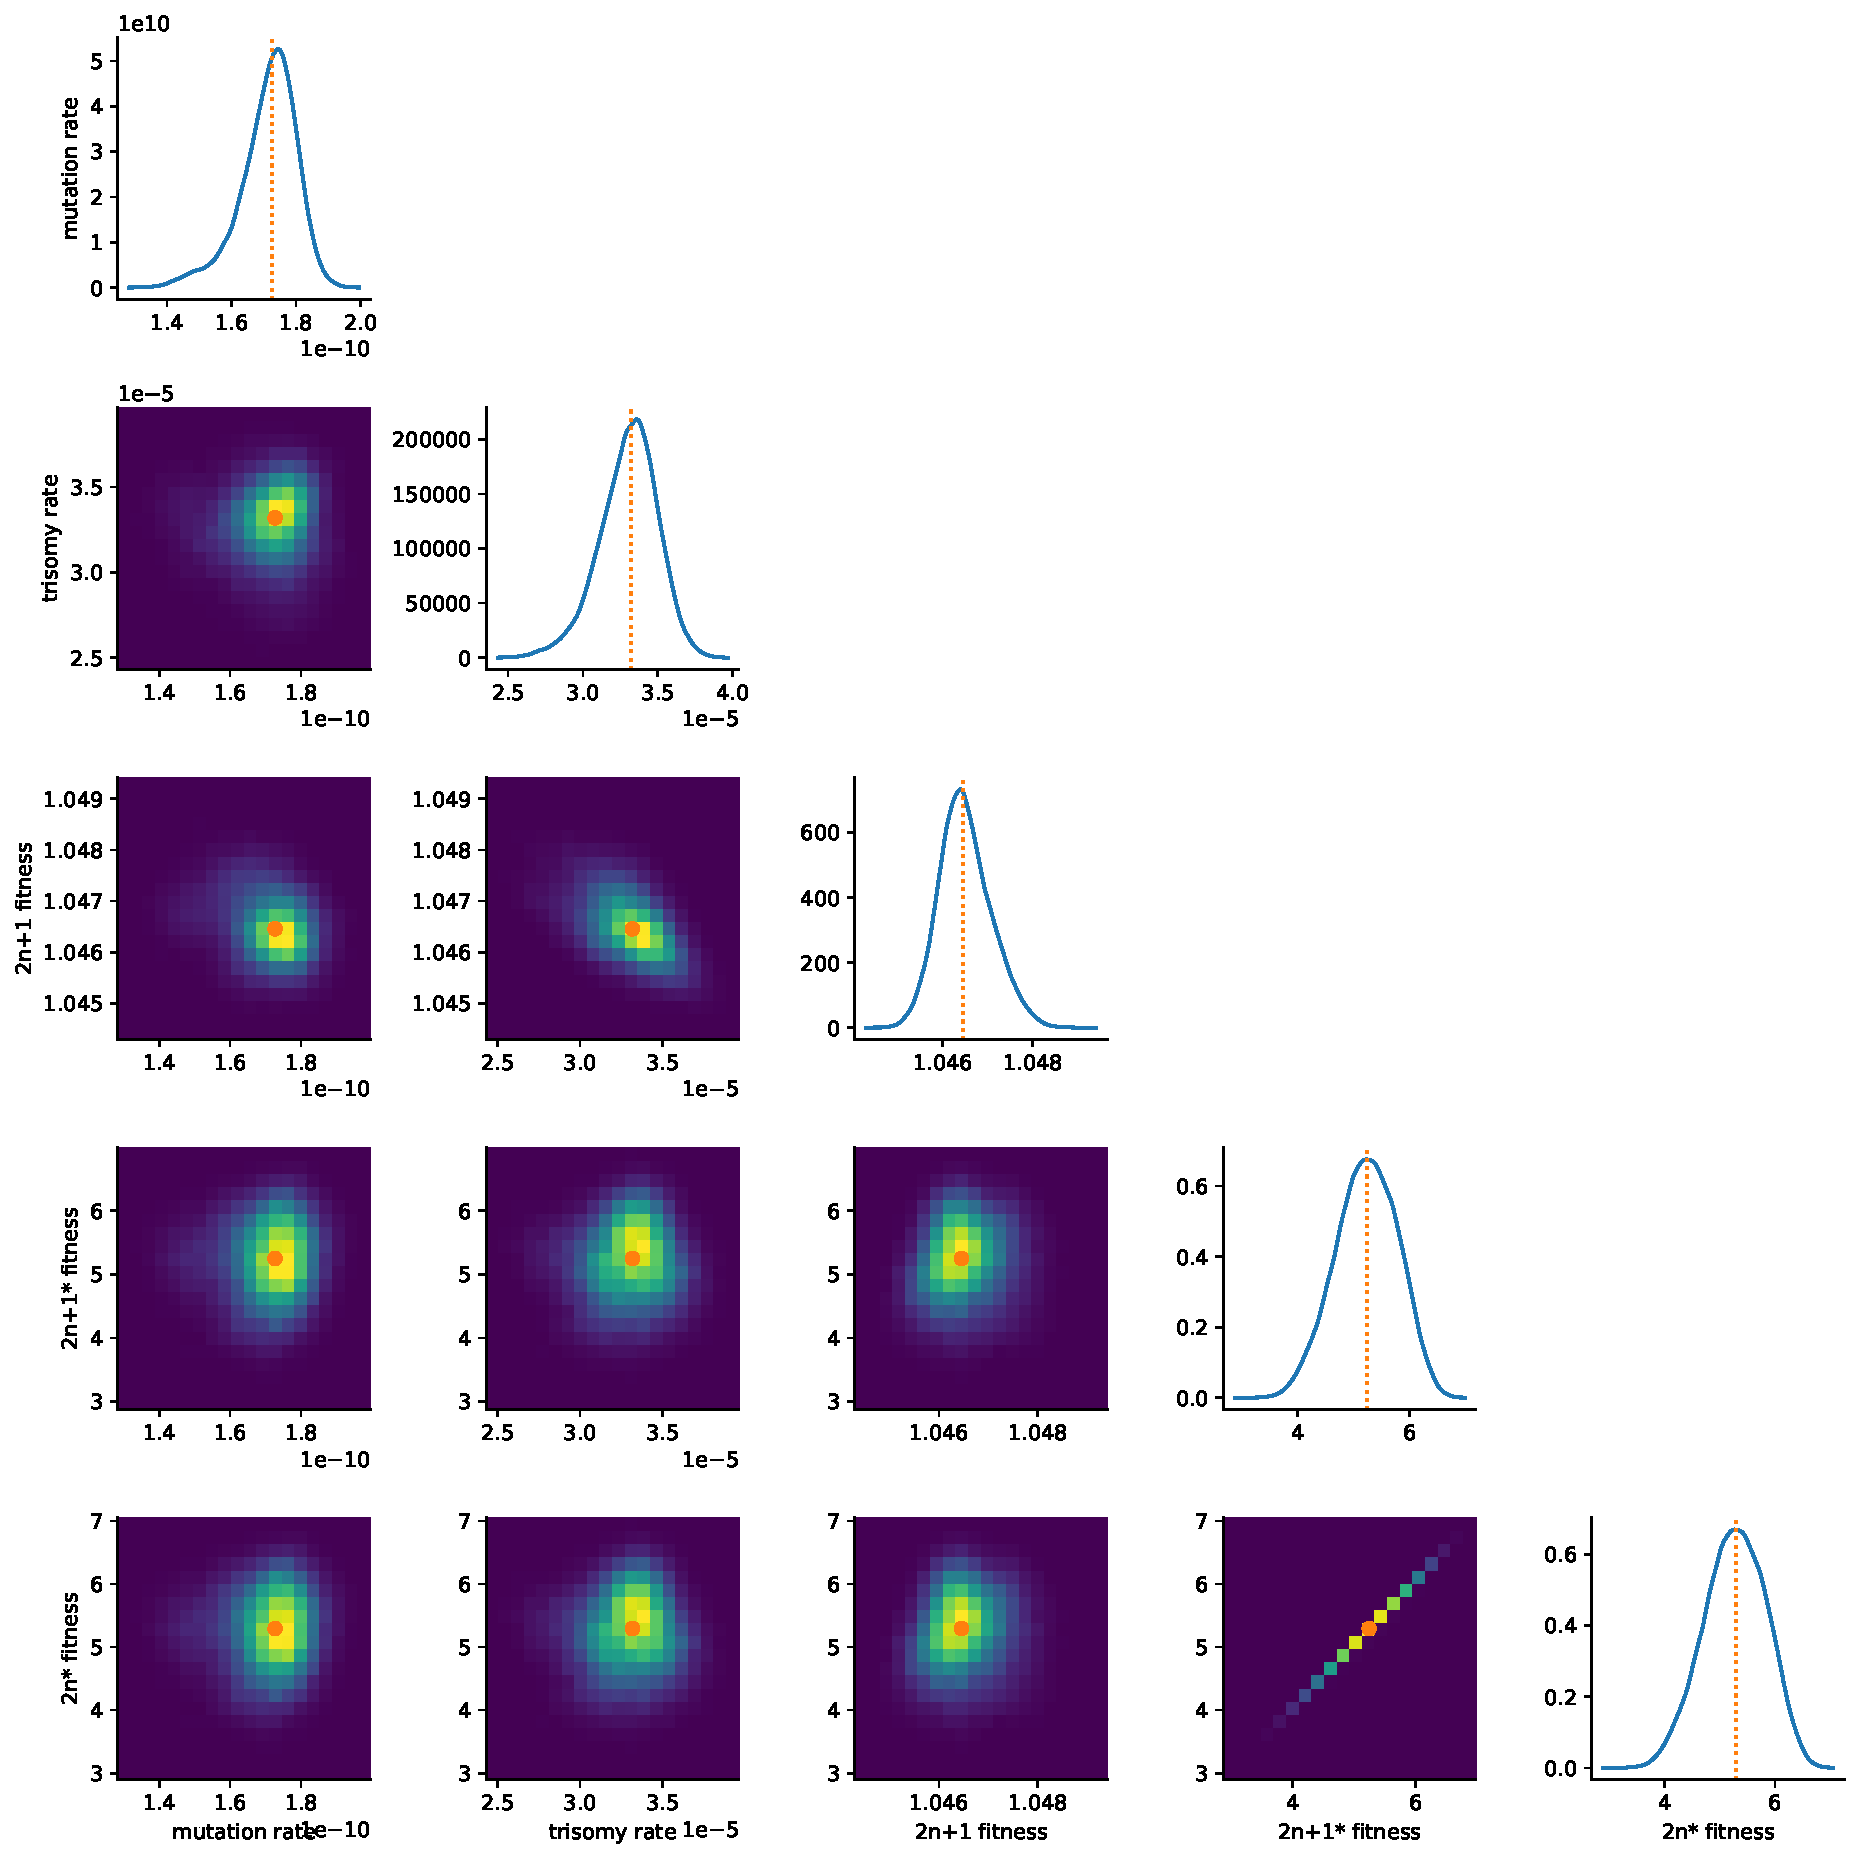
\includegraphics[width=0.9\textwidth]{../figures/posterior.pdf}
  \caption{
  \textbf{Posterior distribution of single-locus model.}
On the diagonal, the inferred posterior distribution of each model parameter. 
Below the diagonal, the inferred joint posterior distribution of pairs of model parameters (dark purple and bright yellow for low and high density, respectively). Red markers and orange lines for the joint MAP estimate (which may differ from the marginal MAP, as the marginal distribution integrates over all other parameters).
} 
  \label{fig:posterior}
\end{figure}
%%%%%%%%%%%%%%%%%%%%%%


\paragraph{Model checking and comparison.}
The single-locus model fits the data well: in simulations using the best-fit parameters (MAP estimate) \eumt\ fixed in 61\% of simulations by generation 1,700 and in 100\% of simulations by generation 2,350~(\autoref{fig:2n*-fixation}-B) and \anwt\ fixed in roughly 300 generations on average (green lines in \autoref{fig:ppc-plot}), which agrees with experimental results.
% TODO replace "roughly 300" with the exact number.
Interestingly, the genotype frequency dynamics in these simulations demonstrate that \anmt\ never reaches substantial frequency (\autoref{fig:ppc-plot}). % TODO move somewhere else?
Furthermore, sensitivity analysis shows that changing the parameter values from the MAP estimate reduces the model fit to the experimental results~(\autoref{fig:sensitivity}).

However, a model without aneuploidy where the aneuploidy rate is fixed at zero, $\delta=0$, cannot explain the experimental observations~(Figure~\ref{fig:2n*-fixation}). The estimated parameter values without aneuploidy are: 
%% generated with MAP-and-hdi.ipynb
mutation rate, $\mu=7.837\substack{+0.078 \\ -0.123}\times10^{-9}$,
fitness of mutant, $w_{2n^*}=1.013\substack{+0.000 \\ -0.000}$. 
We can see that the mutation rate estimate in this model is much lower than in the model with aneuploidy. Higher mutation rate would cause quicker fixation of \eumt\ than in the experimental observations (\autoref{fig:2n*-fixation}). Thus, even disregarding the appearance of trisomic cells in the experiment, the evidence supports the inclusion of aneuploidy in the model.
% TODO WAIC?

% Fig single-locus model with and without aneuploidy
%% generated with with-aneuploidy_vs_no_aneuploidy.ipynb
\begin{figure}[h!]
  \begin{subfigure}{0.5\textwidth}
      \centering
      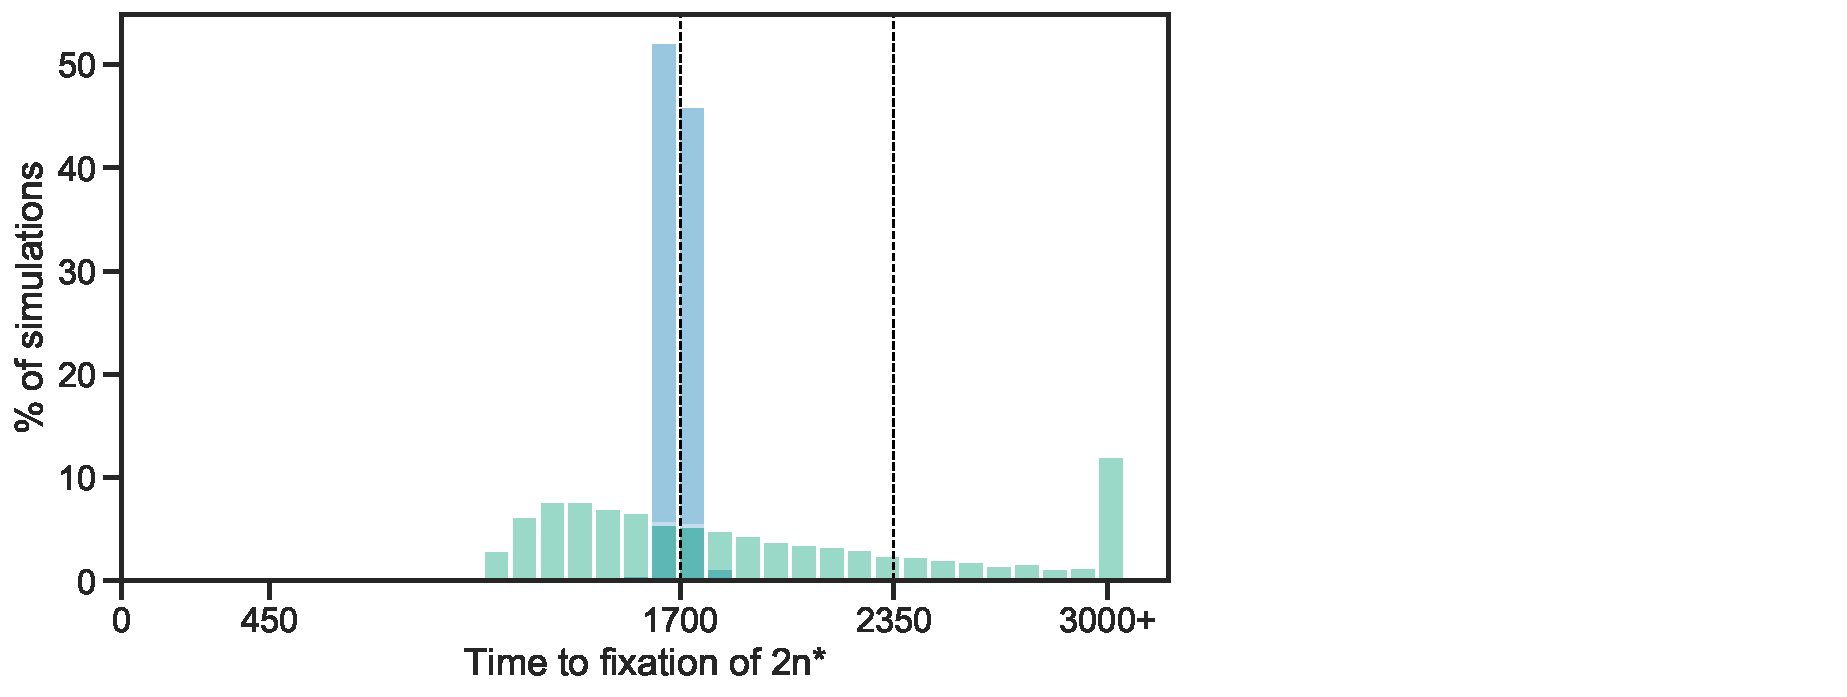
\includegraphics[width=\textwidth]{../figures/fixation-plot-a.pdf}      
      \label{fig:fit}
  \end{subfigure}
  \begin{subfigure}{0.5\textwidth}
      \centering
      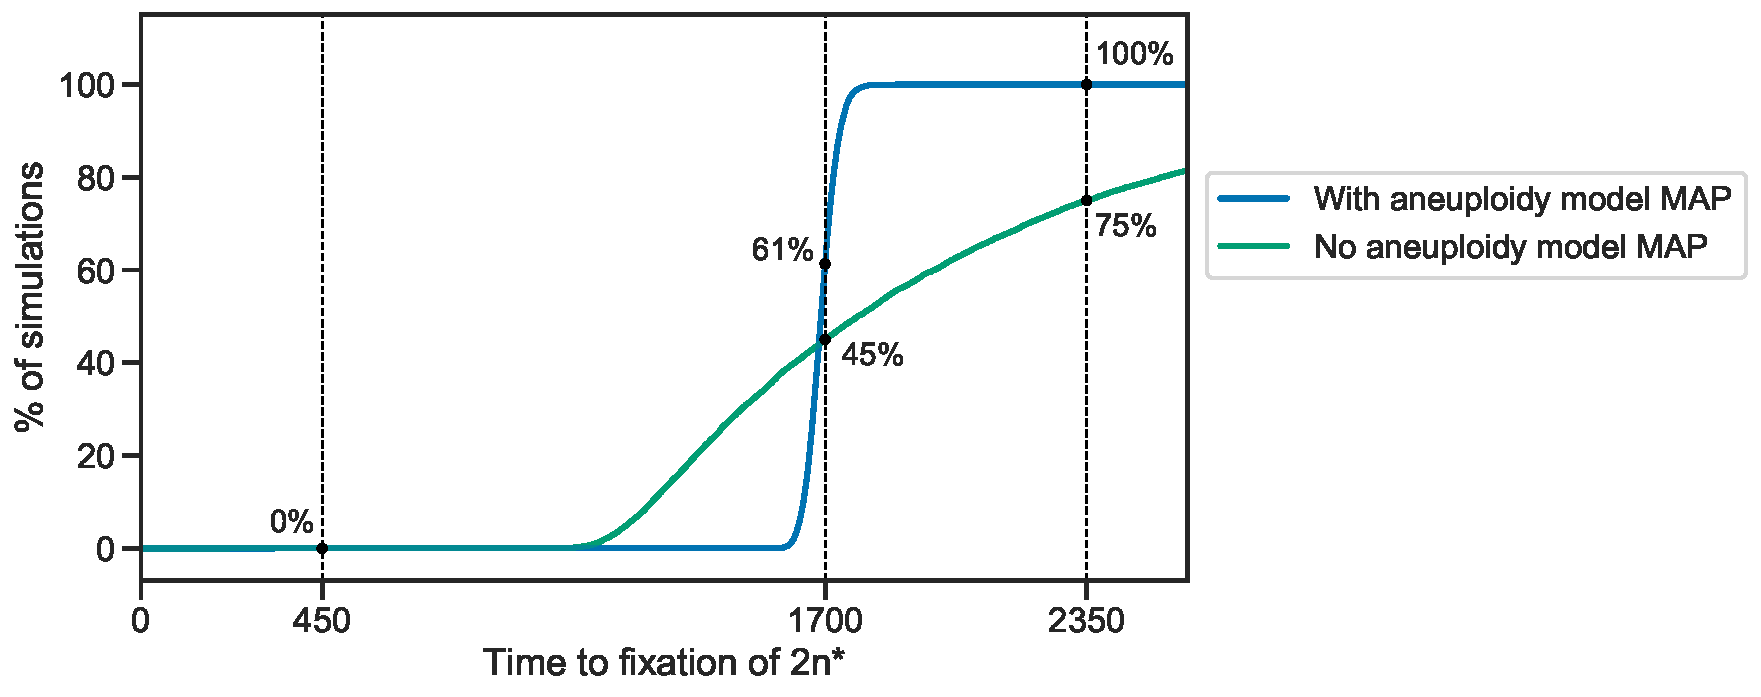
\includegraphics[width=\textwidth]{../figures/fixation-plot-b.pdf}      
      \label{fig:fit-cumulative}
  \end{subfigure}
  \caption{
    \textbf{Single-locus model fit with and without aneuploidy.}
    \textbf{(A)} The distribution of time to fixation of \eumt\ (i.e., adaptation time) in $10,000$ simulations of the single-locus model with aneuploidy (blue; MAP parameters) compared to two models without aneuploidy: a model with the same parameter values except $\delta=0$ (orange), and a model fitted to the data assuming $\delta=0$ (green).
In the experiment by \citet{Yona2012}, one population lost aneuploidy by generation 1,700 and another by generation 2,350 (dashed lines) but not before generation 450. Thus, the blue distribution is a better fit compared to the green, and the yellow histogram has a very poor fit.
The last bin contains all the simulations with time equal or greater than 3,000.
    \textbf{(B)}
	Cumulative distribution of the time to fixation of \eumt\ in 10,000 simulations using the MAP estimate with and without aneuploidy in blue and green, respectively, and corresponding to the blue and green bars in panel A. The MAP likelihood (\autoref{eq:heatstress-likelihood}) is 0.84 and 0.67 with and without aneuploidy, respectively.
     }
  \label{fig:2n*-fixation}
\end{figure}

\begin{figure}[h!]
  \centering
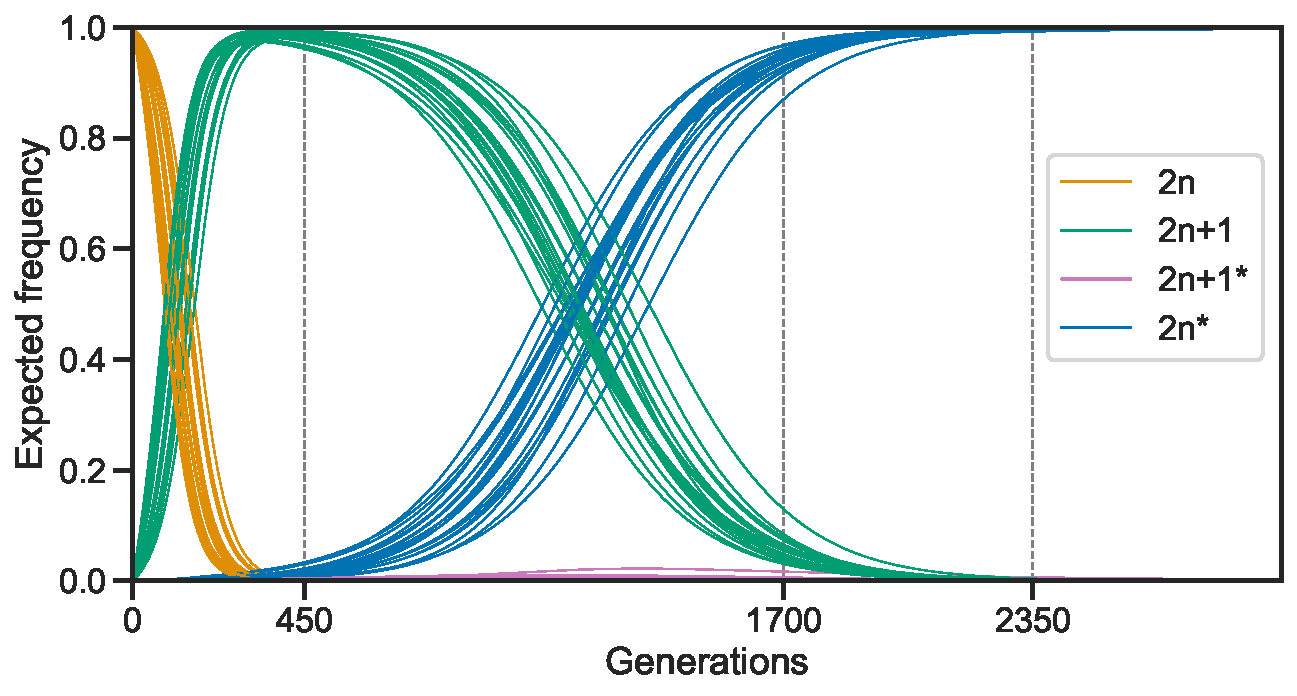
\includegraphics[width=0.8\textwidth]{../figures/dynamics.pdf}
  \caption{
  \textbf{Posterior genotype frequency dynamics for the single-locus model.} 
  The posterior prediction for the frequencies of the four genotypes over time. Each of the 20 curves is the average of 10,000 simulations of the single-locus model using parameters drawn from the posterior distribution.
  }
  \label{fig:ppc-plot}
\end{figure}

% Fig tau comparisons
%% generated with diff-tau.ipynb
\begin{figure}[h!]
  \centering
  \begin{subfigure}{0.45\textwidth}
      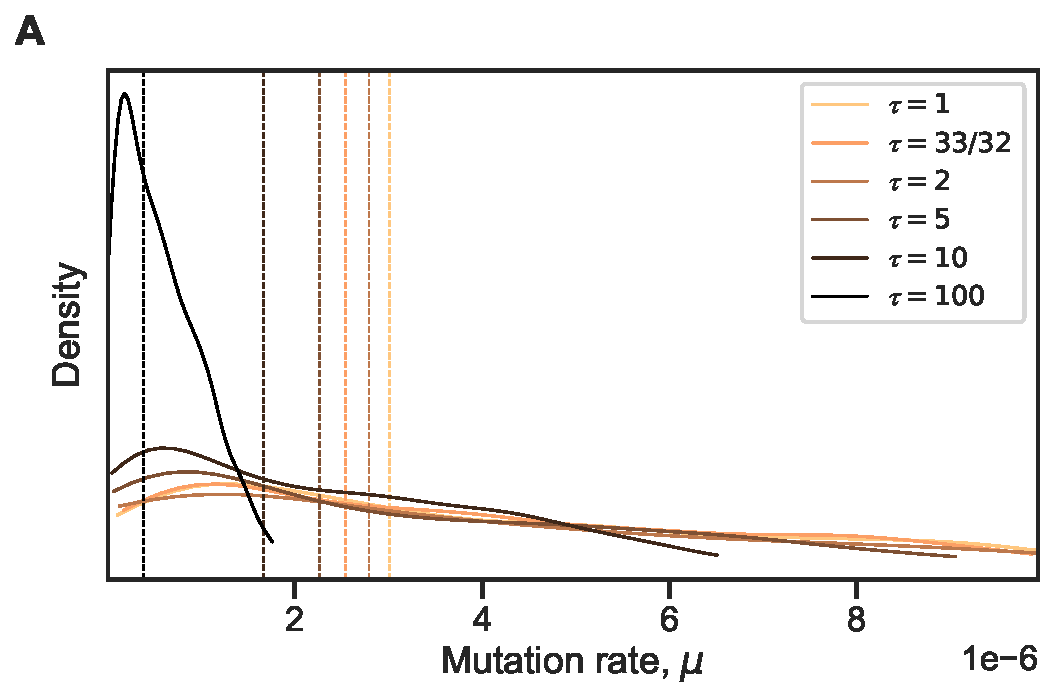
\includegraphics[width=\textwidth]{../figures/tau-A.pdf}      
  \end{subfigure}
  \begin{subfigure}{0.45\textwidth}
      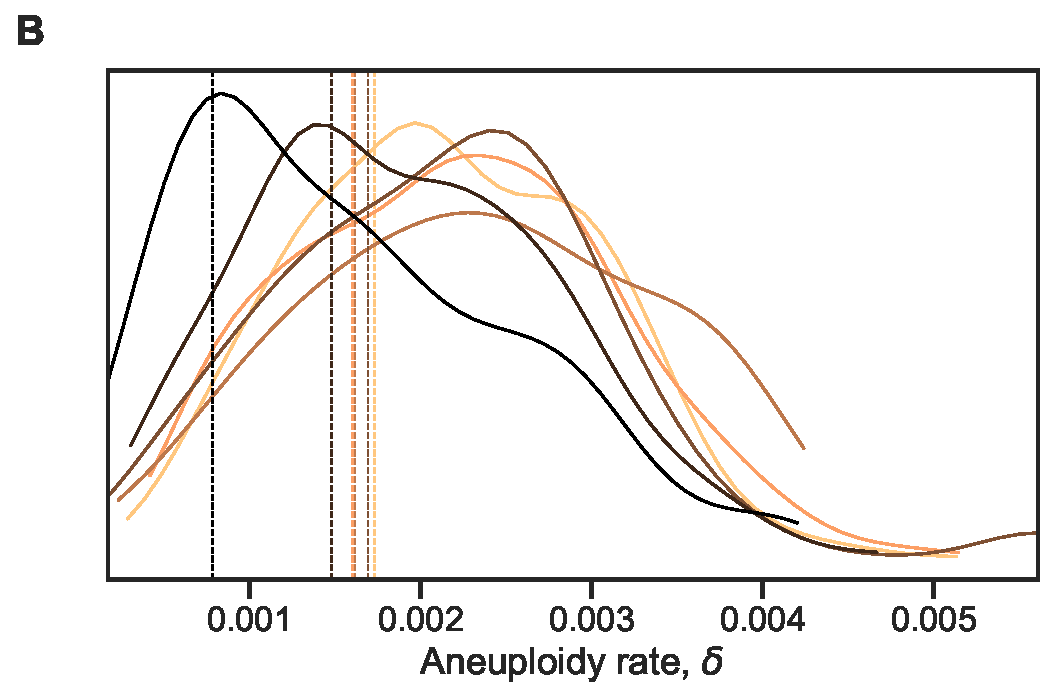
\includegraphics[width=\textwidth]{../figures/tau-B.pdf}      
  \end{subfigure}
  \\
   \begin{subfigure}{0.325\textwidth}
      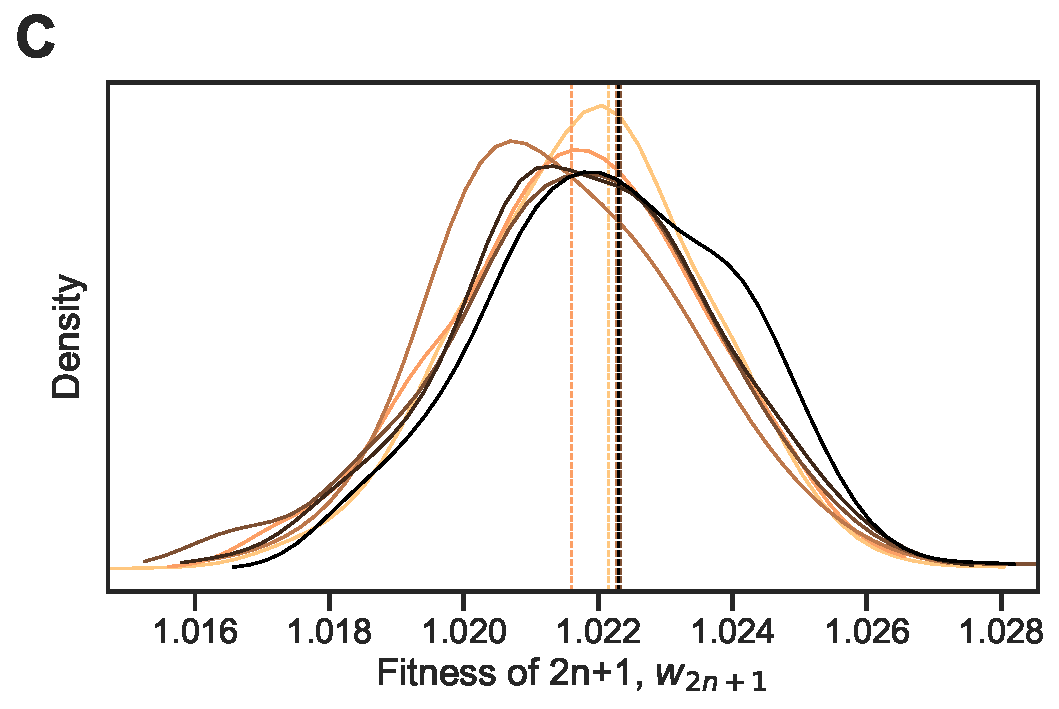
\includegraphics[width=\textwidth]{../figures/tau-C.pdf}      
  \end{subfigure}
    \begin{subfigure}{0.325\textwidth}
      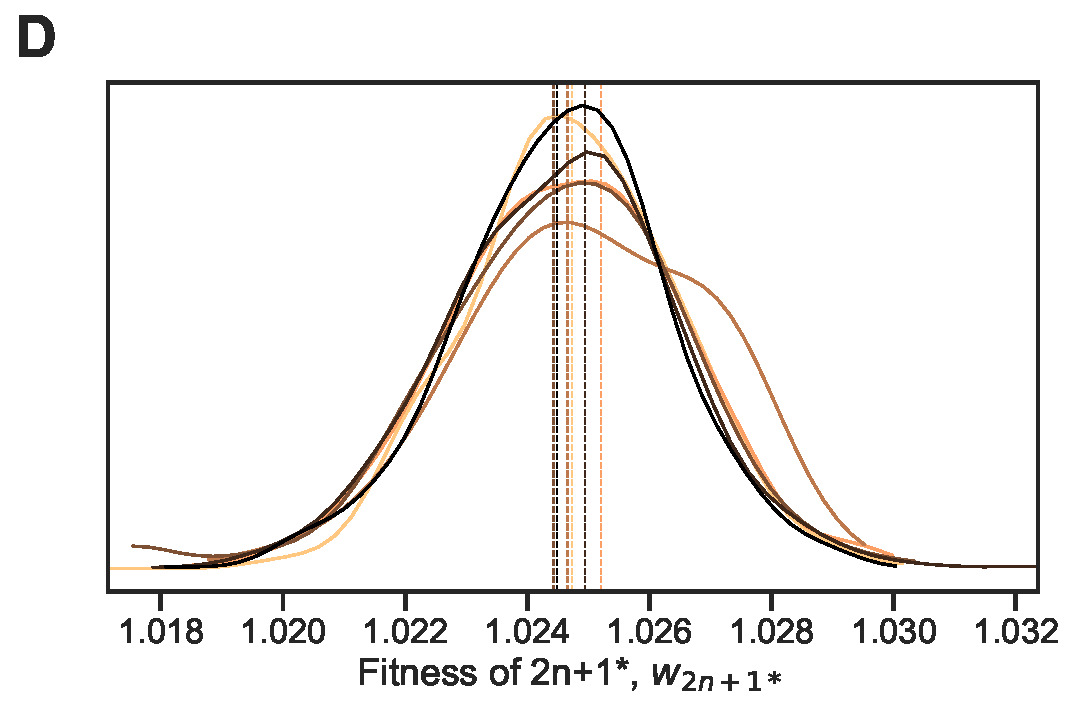
\includegraphics[width=\textwidth]{../figures/tau-D.pdf}      
  \end{subfigure}
    \begin{subfigure}{0.325\textwidth}
      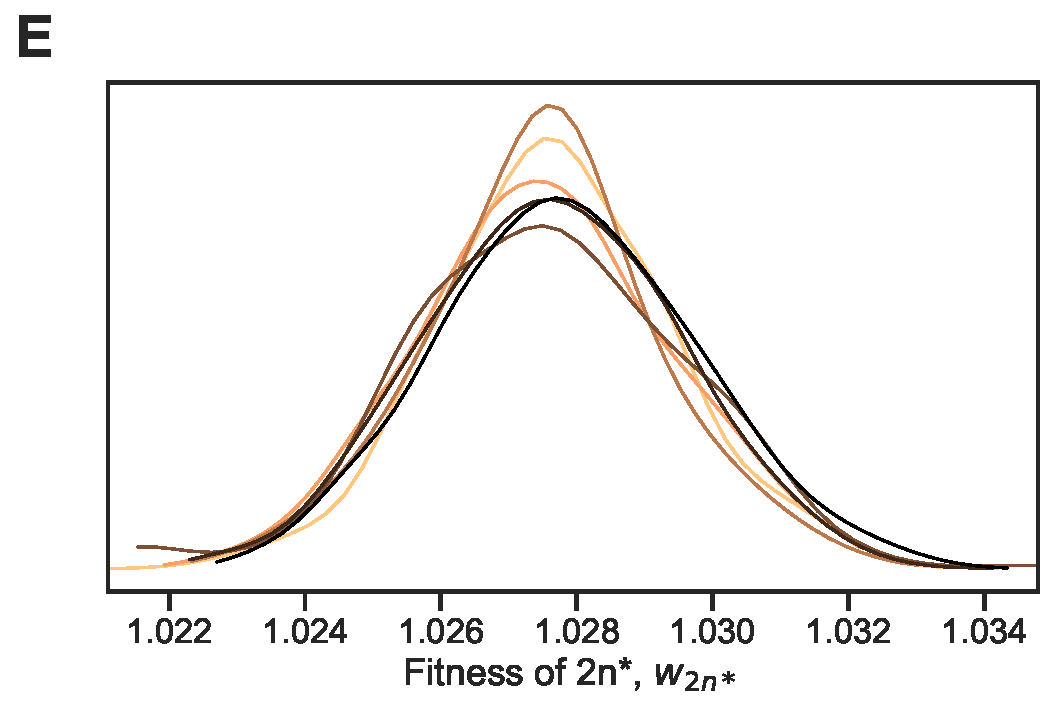
\includegraphics[width=\textwidth]{../figures/tau-E.pdf}      
  \end{subfigure}
  \\
  \begin{subfigure}{0.325\textwidth}
      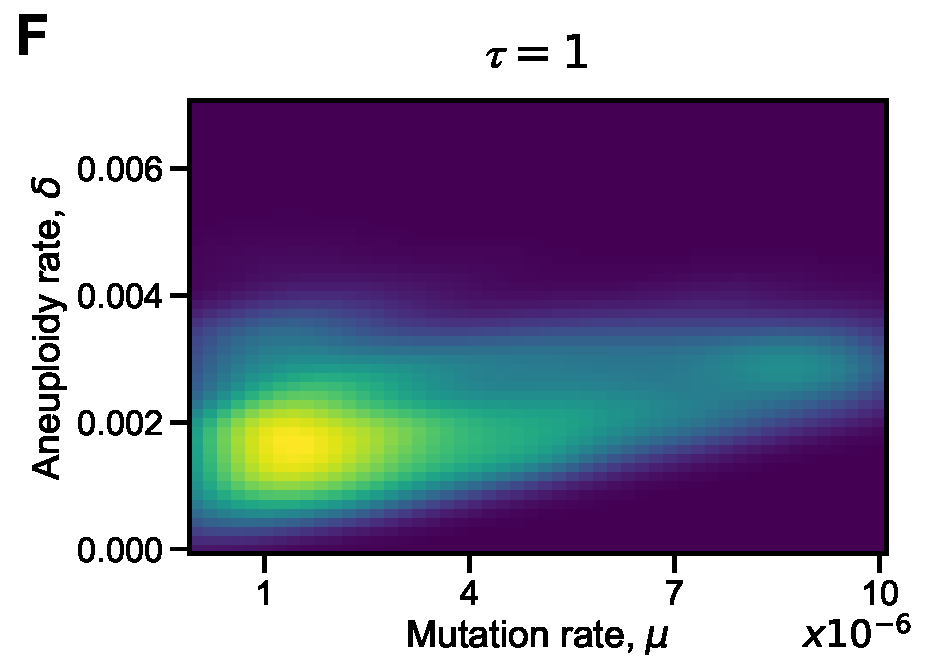
\includegraphics[width=\textwidth]{../figures/tau-joint-F.pdf}      
  \end{subfigure}
\begin{subfigure}{0.325\textwidth}
      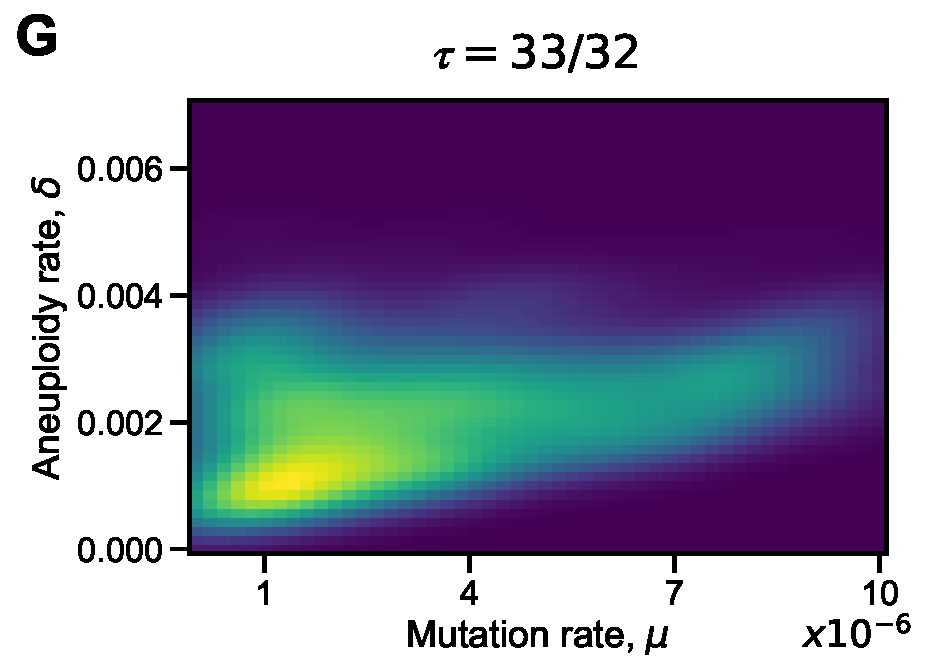
\includegraphics[width=\textwidth]{../figures/tau-joint-G.pdf}      
  \end{subfigure}
\begin{subfigure}{0.325\textwidth}
      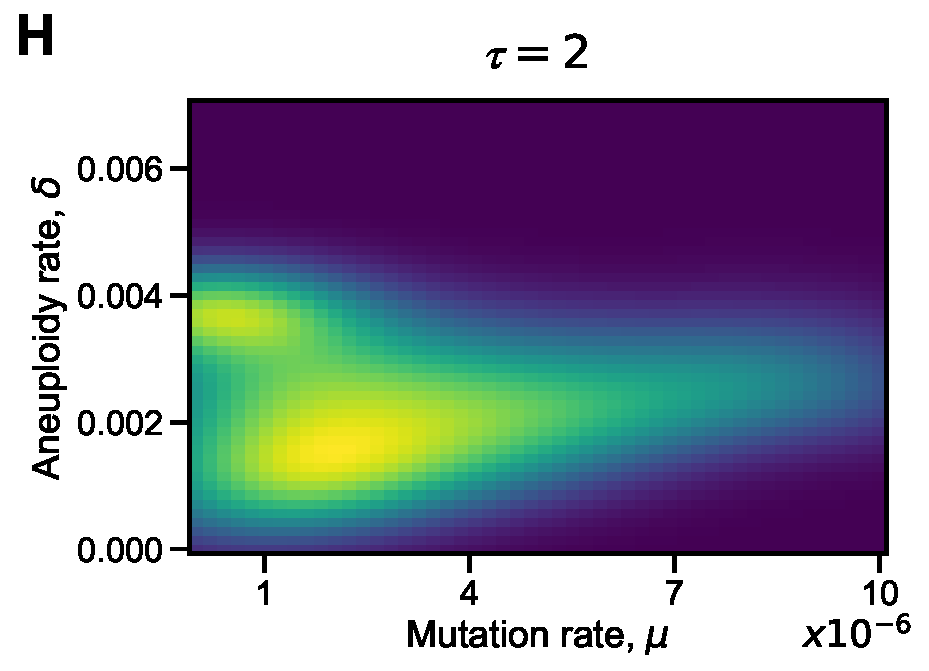
\includegraphics[width=\textwidth]{../figures/tau-joint-H.pdf}      
  \end{subfigure}
\begin{subfigure}{0.325\textwidth}
      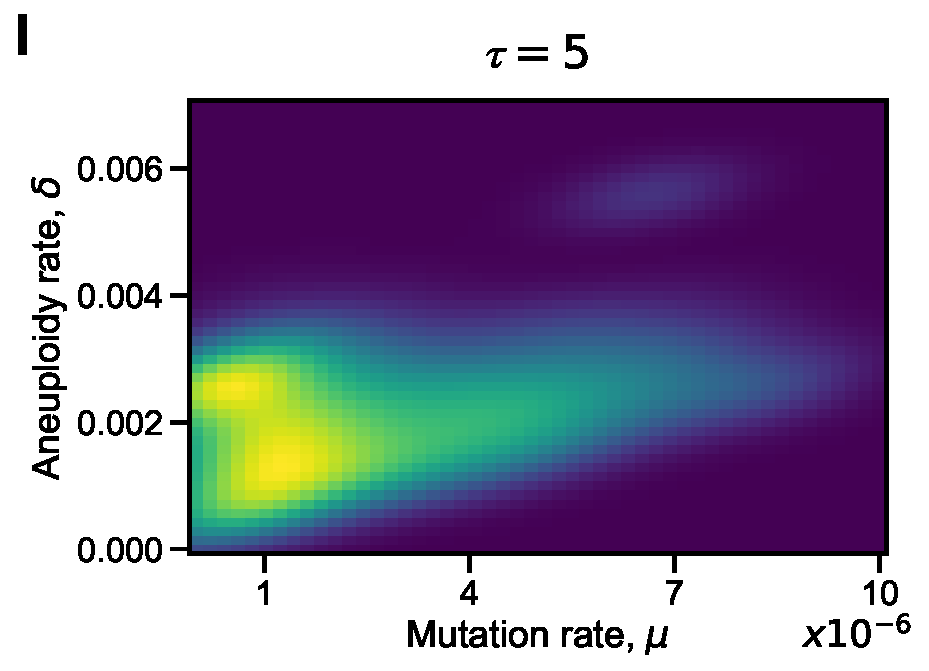
\includegraphics[width=\textwidth]{../figures/tau-joint-I.pdf}      
  \end{subfigure}
\begin{subfigure}{0.325\textwidth}
      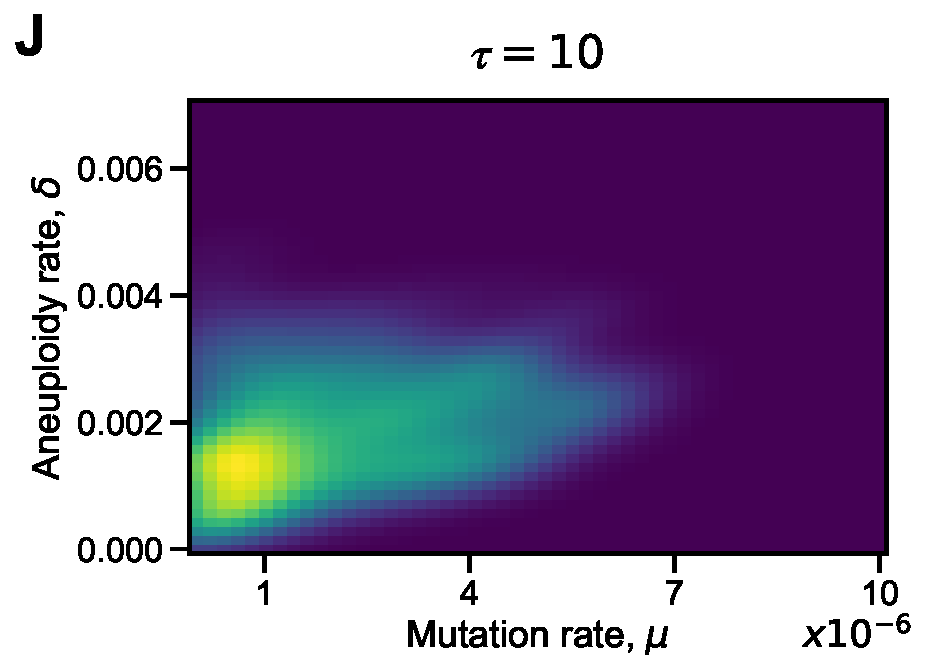
\includegraphics[width=\textwidth]{../figures/tau-joint-J.pdf}      
  \end{subfigure}
\begin{subfigure}{0.325\textwidth}
      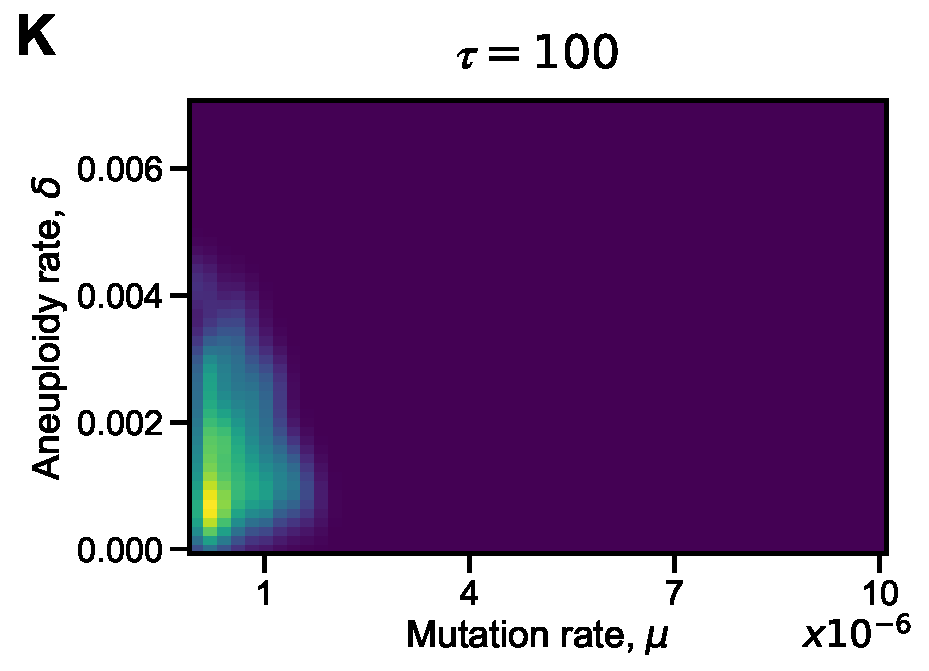
\includegraphics[width=\textwidth]{../figures/tau-joint-K.pdf}      
  \end{subfigure}
  \caption{
    \textbf{Single-locus model with different $\tau$ comparison.}  \textbf{(A-E)} The inferred posterior distribution of each model paramter for the single-locus model with different $\tau$. For $\tau=10$ and $\tau=100$ the mutation and aneuploidy rates tends to be lower.  \textbf{(F-K)} The inferred joint posterior distribution of mutation rate and aneuploidy rate for the single locus model with different $\tau$ (dark purple and bright yellow for low and high density, respectively).
  \label{fig:tau}
  }
  \end{figure}


\paragraph{Inference: multi-locus model.}

%TODO same for complex model
%model comparison between models - model probabilities

\pagebreak
% Discussion
\section*{Discussion}

\paragraph*{Aneuploidy is not just another type of mutation.}
The published data indicate that, like mutation, aneuploidy can be both deleterious and beneficial~\citep{Pavelka2010, Sheltzer2011}.
Nevertheless, there are important and fundamental differences between adaptation by aneuploidy
and adaptation by beneficial mutations~\citep{Yona2015}, which make aneuploidy a unique mechanism for generating genetic
variation.
First, the aneuploidy rate (i.e. the frequency of mis-segregation events) is significantly higher than the
mutation rate~\citep{Santaguida2015review}.
Thus, everything else being equal, adaptation by aneuploidy will be faster and more frequent.
Second, fitness effects of aneuploidy are larger than those of the majority of mutations, on average, and are rarely
neutral~\citep{Pavelka2010, Yona2012, Sunshine2015}, allowing selection to quickly sort deleterious and beneficial genotypes.
Third, the number of different karyotypes is considerably smaller than the number of different genotypes, and different karyotypes are likely to have different phenotypes~\citep{Pavelka2010}.
Therefore, exploration of the phenotype space by aneuploidy requires smaller populations and a shorter time span.
Fourth, aneuploidy is a reversible state, as the rate of chromosome loss is high and the cost of aneuploidy is significant~\citep{Niwa2006}.
Indeed, aneuploidy often provides a transient solution: under short-term stress conditions, aneuploidy reverts (chromosome number returns to normal) when the stress subsides; under long-term stress conditions, aneuploidy reverts when refined solutions, generated by beneficial mutations, take over~\citep{Yona2012}.
Finally, aneuploidy results in increased genome instability, potentially increasing genetic variation by a positive feedback loop~\citep{Rancati2013, Bouchonville2009, Zhu2012}, while also increasing its own transience.

\paragraph*{Evolutionary theory of aneuploidy.}
The role of aneuploidy in adaptation has only recently been observed~\citep{Sionov2010, Yona2012, Gerstein2015}, and is largely missing from the literature on evolution and adaptation:
the introductory textbook \emph{Evolution} by~\citet{Bergstrom2012} does not mention the word aneuploidy, and the graduate-level book \emph{Mutation-Driven Evolution} by~\citet{Nei2013} only briefly mentions aneuploidy in the context of speciation, but not adaptation.
In recent reviews of the literature, aneuploidy is suggested to play an important role in fungal adaptation~\citep{Robbins2017, Todd2017} and cancer evolution~\citep{Santaguida2015review, Naylor2016, Sansregret2017}, yet these reviews cite no theoretical studies nor any quantitative models.
Indeed, evolutionary, ecological, and epidemiological studies mostly assume adaptation occurs via beneficial mutations, recombination, and sex.
Therefore, there is a critical need to develop an evolutionary theory of aneuploidy like the evolutionary theories of other mechanisms for generation of genetic variation, e.g. mutation~\citep{Lynch2010}, recombination~\citep{Hartfield2012}, and sex~\citep{Otto2009}.
An evolutionary theory of aneuploidy will be central to the interpretation of experimental and clinical observations and design of new hypotheses, experiments, and treatments~\citep{Carja2014}.
For example, despite the lack of theoretical models, aneuploidy has been invoked in a new strategy to combat pathogens and tumour cells by setting ``evolutionary traps''~\citep{Gerstein2015,Chen2015}, in which a condition that predictably leads to emergence of aneuploidy is applied, followed by a condition that specifically selects against aneuploid cells.

\pagebreak
% Acknowledgements
{\small
\section*{Acknowledgements}
We thank Yitzhak Pilpel, Orna Dahan, Lilach Hadany, Judith Berman, David Gresham, Shay Covo, Martin Kupiec, and Tal Simon for discussions and comments.
This work was supported in part by 
the Israel Science Foundation (YR 552/19) and
Minerva Stiftung Center for Lab Evolution (YR).
% TODO add Minerva for Martin; funding for Avihu?
}

\bibliographystyle{agsm}
\bibliography{ms.bib}

\section*{Supplementary Material}
\beginsupplement % https://support.authorea.com/en-us/article/how-to-create-an-appendix-section-or-supplementary-information-1g25i5a/


\begin{figure}[h]
% Fig Curveball 30deg
% generated with growth_curves.ipynb
\begin{subfigure}{0.5\textwidth}
    \centering
	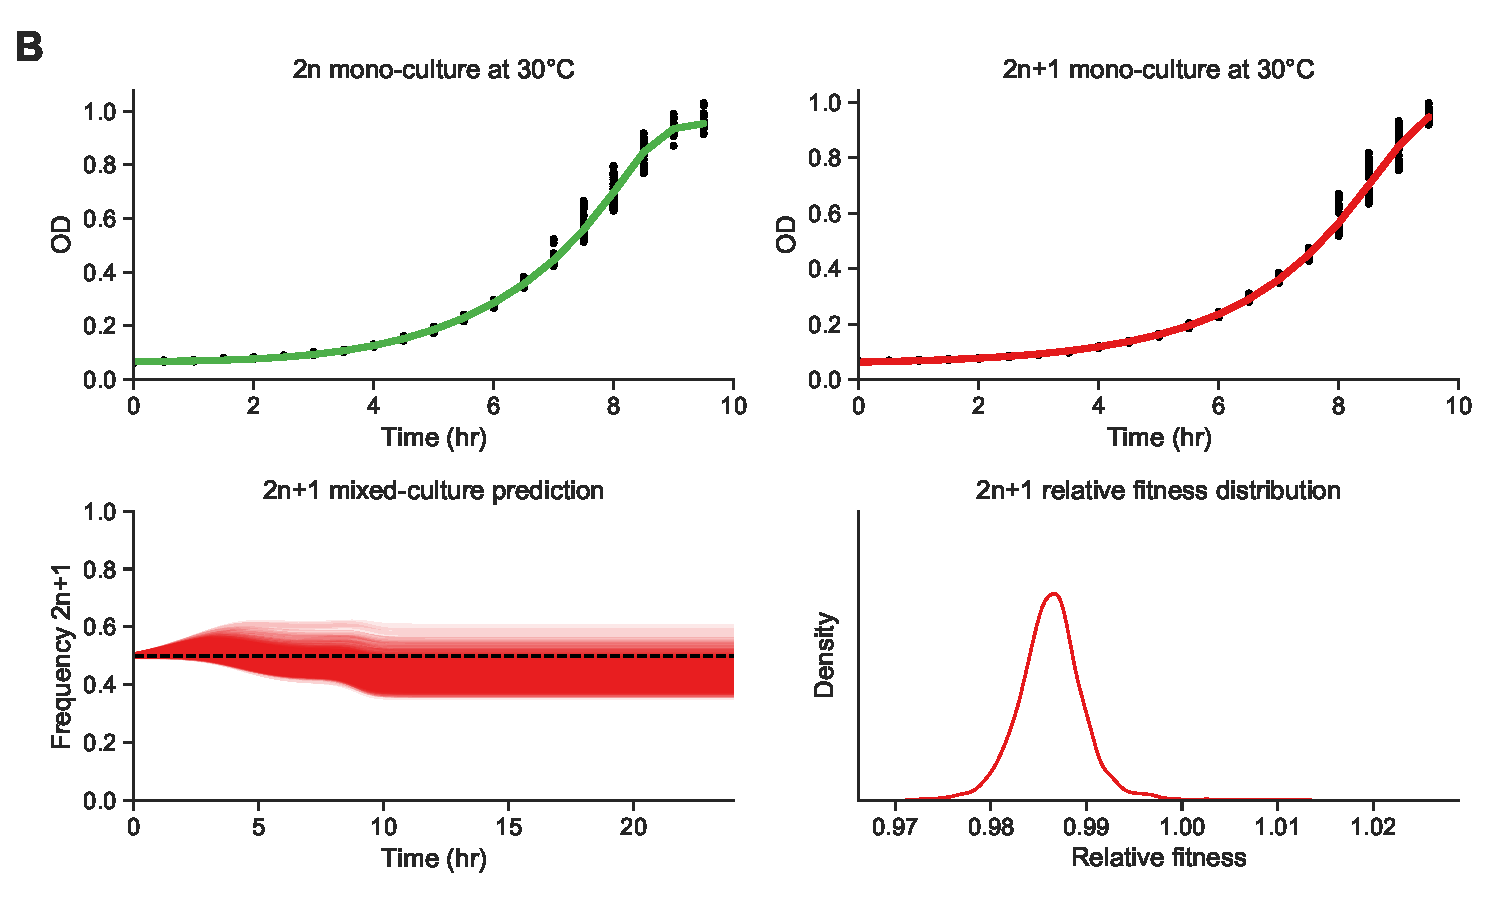
\includegraphics[width=\textwidth]{../figures/evo39_fitness_30deg.pdf}
    \label{fig:growth-curves-30deg}
\end{subfigure}
% Fig Curveball 39deg
% generated with growth_curves.ipynb
\begin{subfigure}{0.5\textwidth}
    \centering
	\includegraphics[width=\textwidth]{../figures/evo39_fitness_39deg.pdf}
    \label{fig:growth-curves-39deg}
\end{subfigure}
\caption{
    \textbf{Fitness estimation from growth curves.}
    \textbf{(A)} Fitness estimation from growth curves collected at \SI{30}.{\celsius}
    \textbf{(B)} Fitness estimation from growth curves collected at \SI{39}.{\celsius}
    Growth curves previously described in \citet[Figs. 3C, 4A, and S2]{Yona2012}.
	Fitness estimated from growth curves using \texttt{Curveball}, a method for predicting results of competition experiments from growth curve data~\citep[\href{https://curveball.yoavram.com}{curveball.yoavram.com}]{Ram2019}. See \emph{Models and Methods, Prior distributions} for more details.
} 
\label{fig:growth-curves}
\end{figure}
%TODO please report here the point estimate and 95% CI for the three distributions, I only have for 1-c+b: 0.9863 (95% CI 0.9790 - 0.9939).
% TODO add panel labels

% Fig likelihood profile
%% generated by sensitivity-analysis.ipynb
\begin{figure}[p]
  \centering
  \begin{subfigure}{0.3\textwidth}
      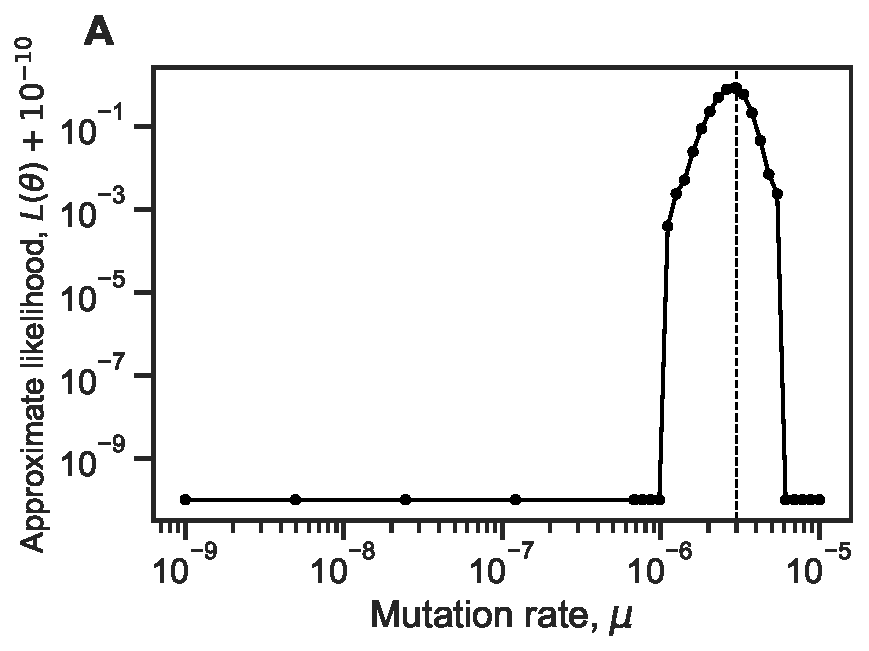
\includegraphics[width=\textwidth]{../figures/sensitivity-A.pdf}      
      \label{fig:sensitivity-mutation}
  \end{subfigure}
  \begin{subfigure}{0.3\textwidth}
      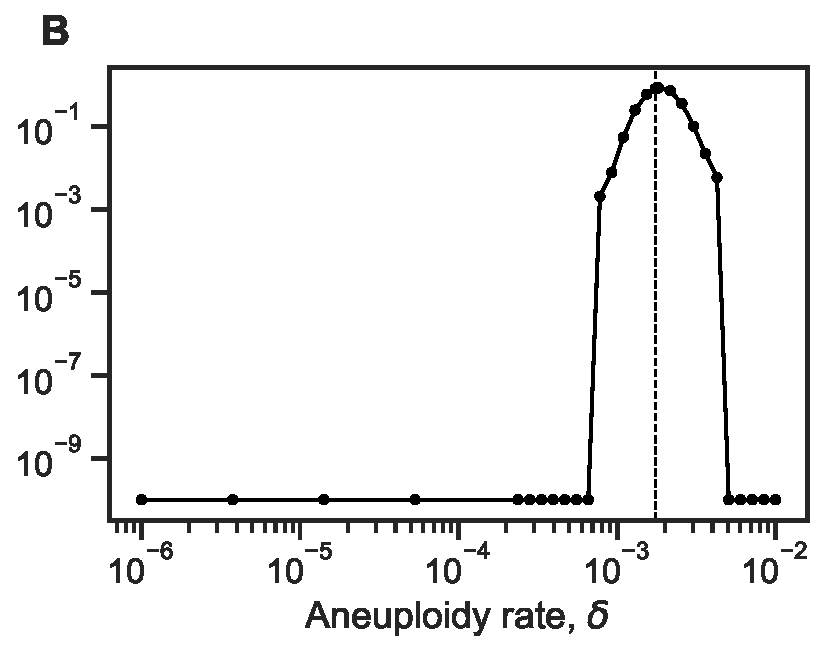
\includegraphics[width=\textwidth]{../figures/sensitivity-B.pdf}      
      \label{fig:sensitivity-aneuploidy}
  \end{subfigure}
  \\
   \begin{subfigure}{0.3\textwidth}
      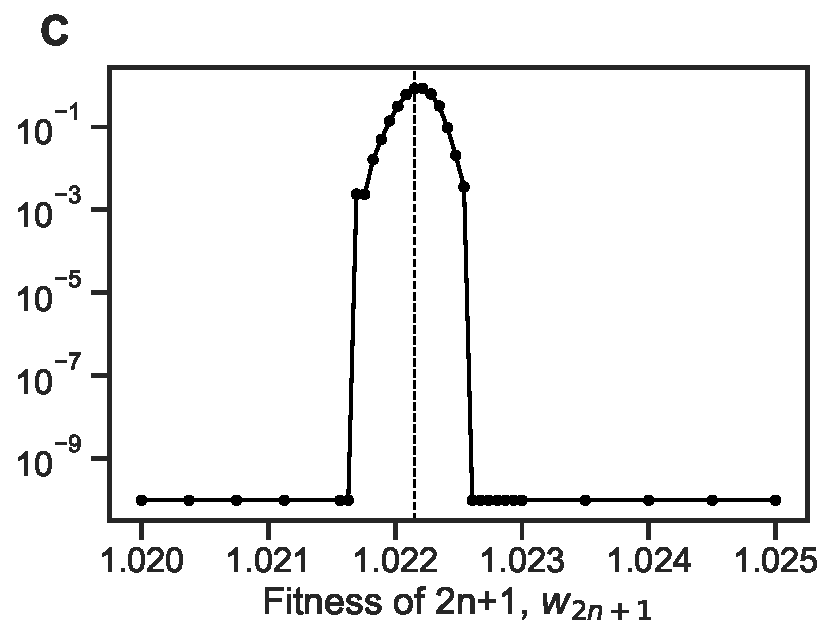
\includegraphics[width=\textwidth]{../figures/sensitivity-C.pdf}      
      \label{fig:sensitivity-anwt}
  \end{subfigure}
    \begin{subfigure}{0.3\textwidth}
      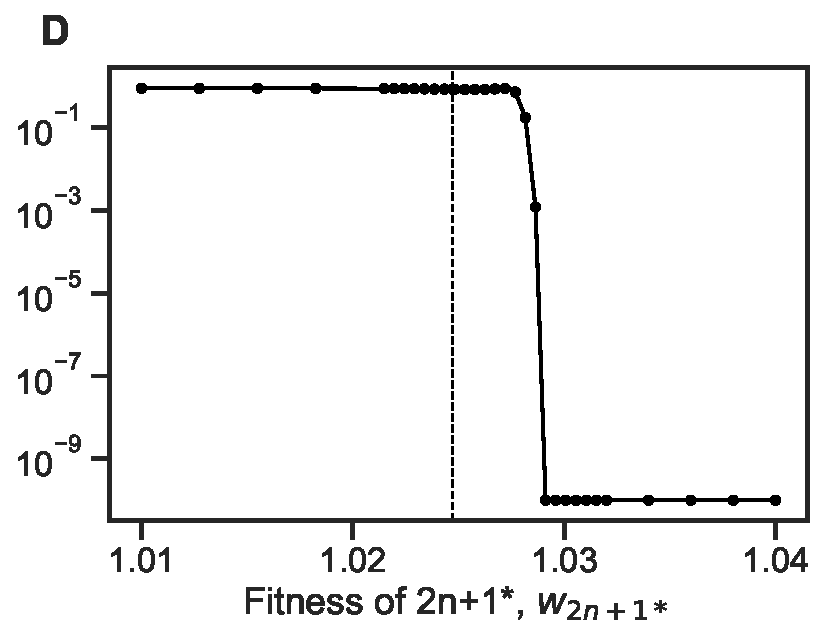
\includegraphics[width=\textwidth]{../figures/sensitivity-D.pdf}      
      \label{fig:sensitivity-anmt}
  \end{subfigure}
    \begin{subfigure}{0.3\textwidth}
      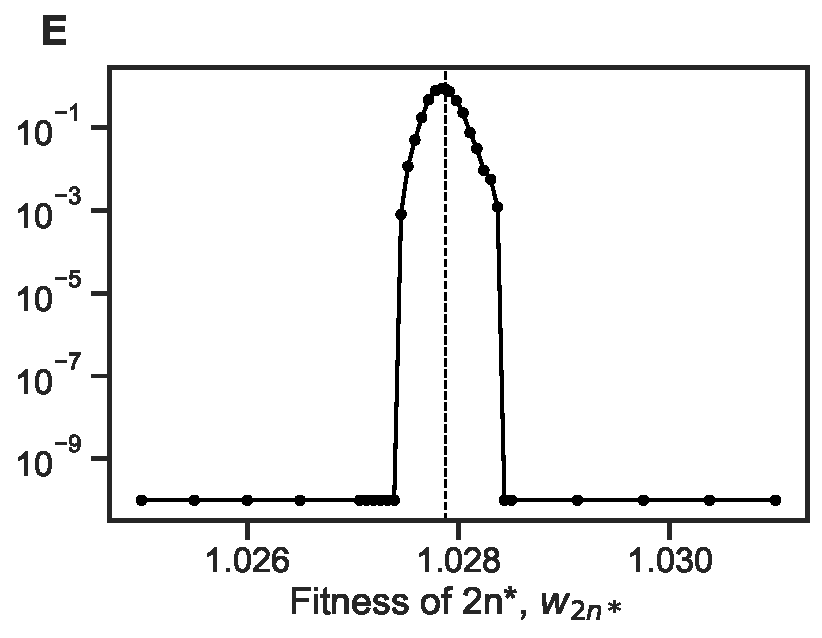
\includegraphics[width=\textwidth]{../figures/sensitivity-E.pdf}      
      \label{fig:sensitivity-eumt}
  \end{subfigure}
  \caption{
    \textbf{Likelihood profiles.} Sensitivity of the approximate likelihood of the single-locus model, $\likelihood(\theta)$, to changing a single parameter while the other parameters remain fixed at their MAP estimates. Dashed vertical line represents the MAP value.
  }
  
  \label{fig:sensitivity}
  % TODO what defines the x range? is it the prior distribution range?
  %ANS: yes for mutation and aneuploidy rates. For fitness just around the MAP in range that looks beautiful.
\end{figure}


% Fig ABC iterations, convergence
%% generated with convergence.ipynb
\begin{figure}[h]

  \begin{subfigure}{1\textwidth}
    \centering
      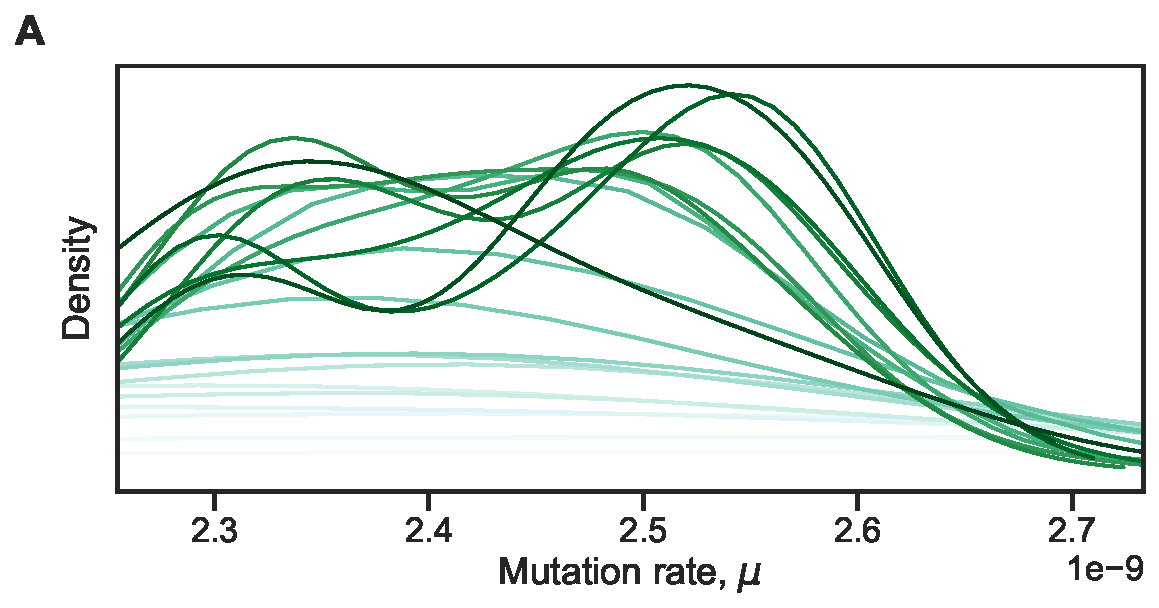
\includegraphics[width=0.45\textwidth]{../figures/convergence-p1_mr.pdf}      
      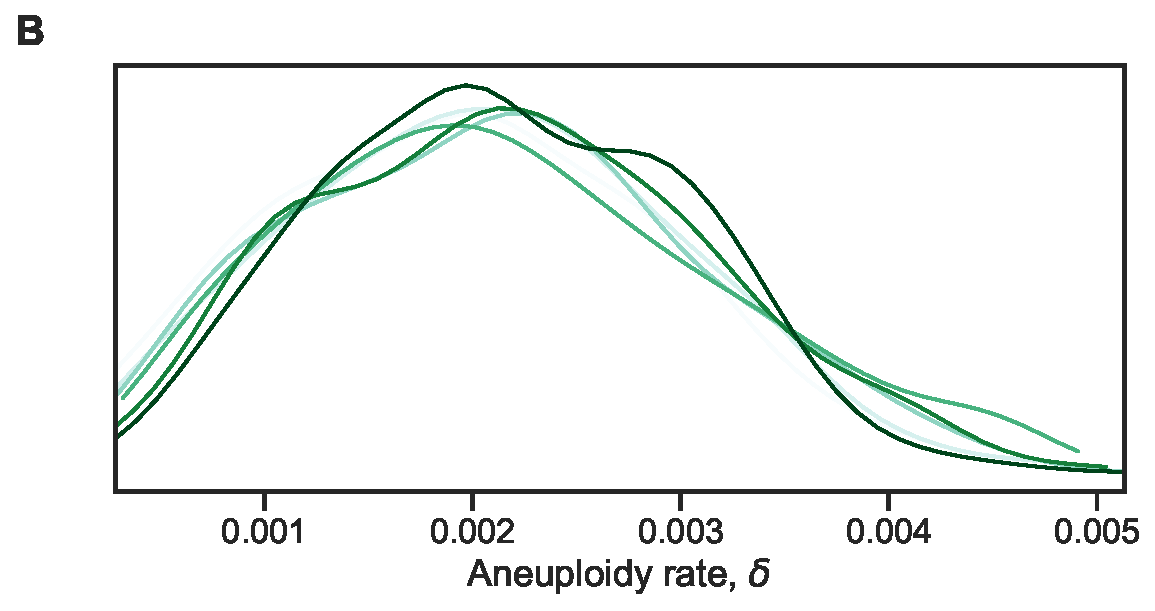
\includegraphics[width=0.45\textwidth]{../figures/convergence-p2_tr.pdf} \\     
      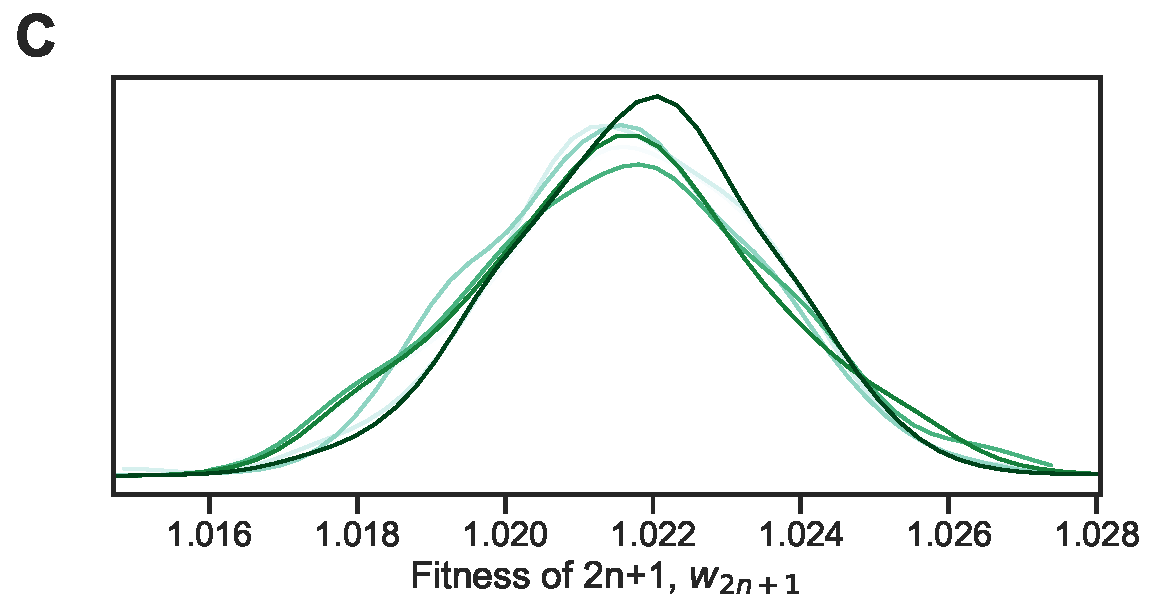
\includegraphics[width=0.325\textwidth]{../figures/convergence-p3_w1.pdf}      
      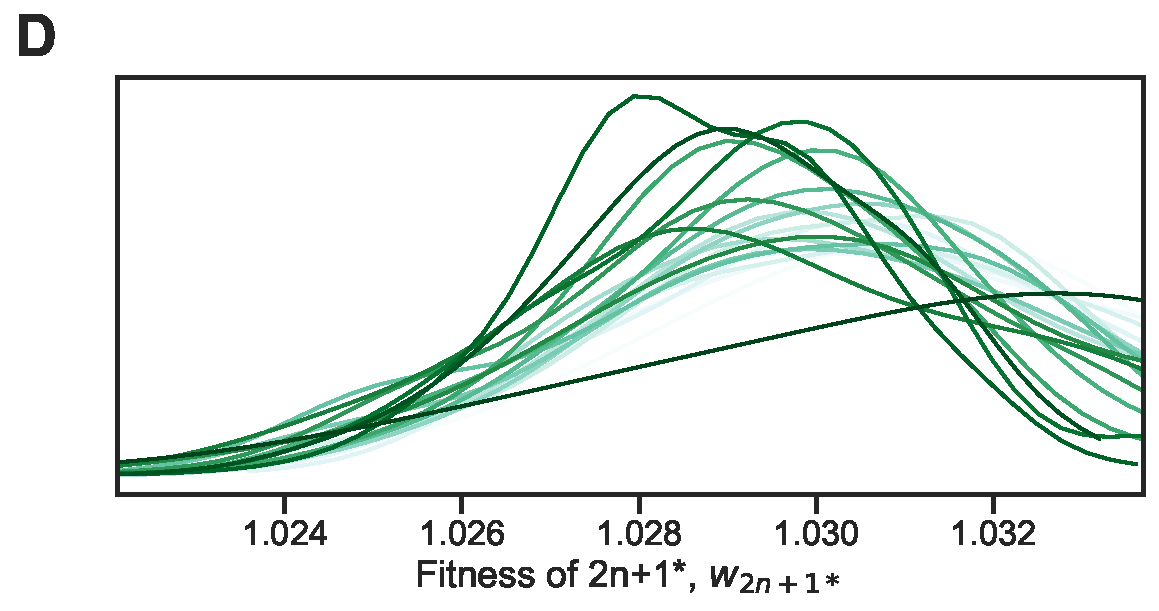
\includegraphics[width=0.325\textwidth]{../figures/convergence-p4_w2.pdf}      
      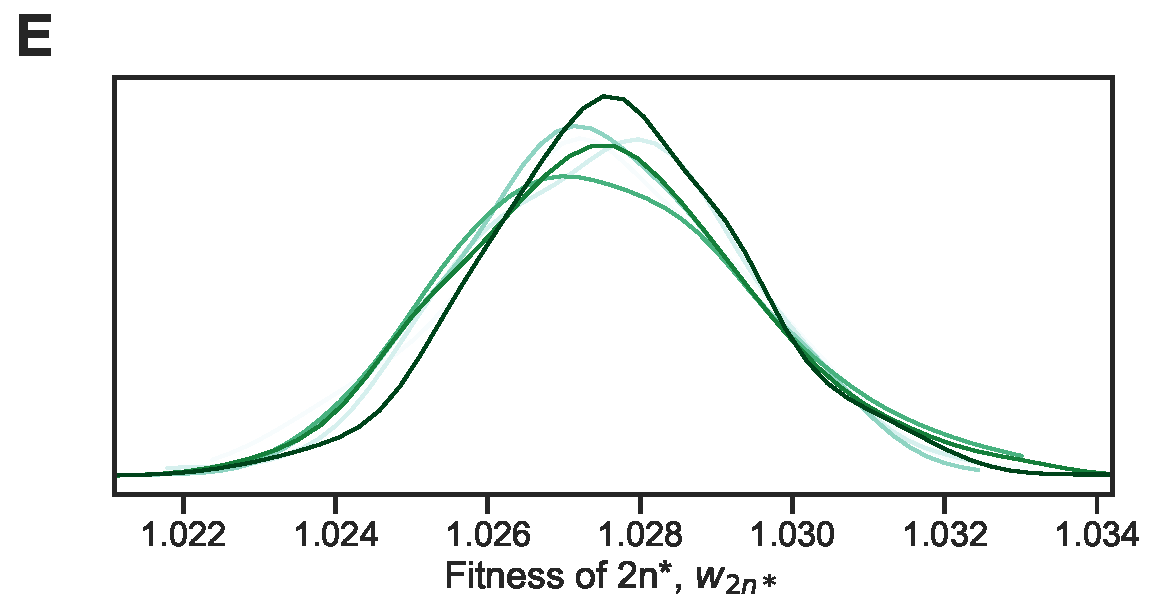
\includegraphics[width=0.325\textwidth]{../figures/convergence-p5_w3.pdf}      
     \label{fig:convergence-A}
    \end{subfigure}
    \\    
  \begin{subfigure}{1\textwidth}
  	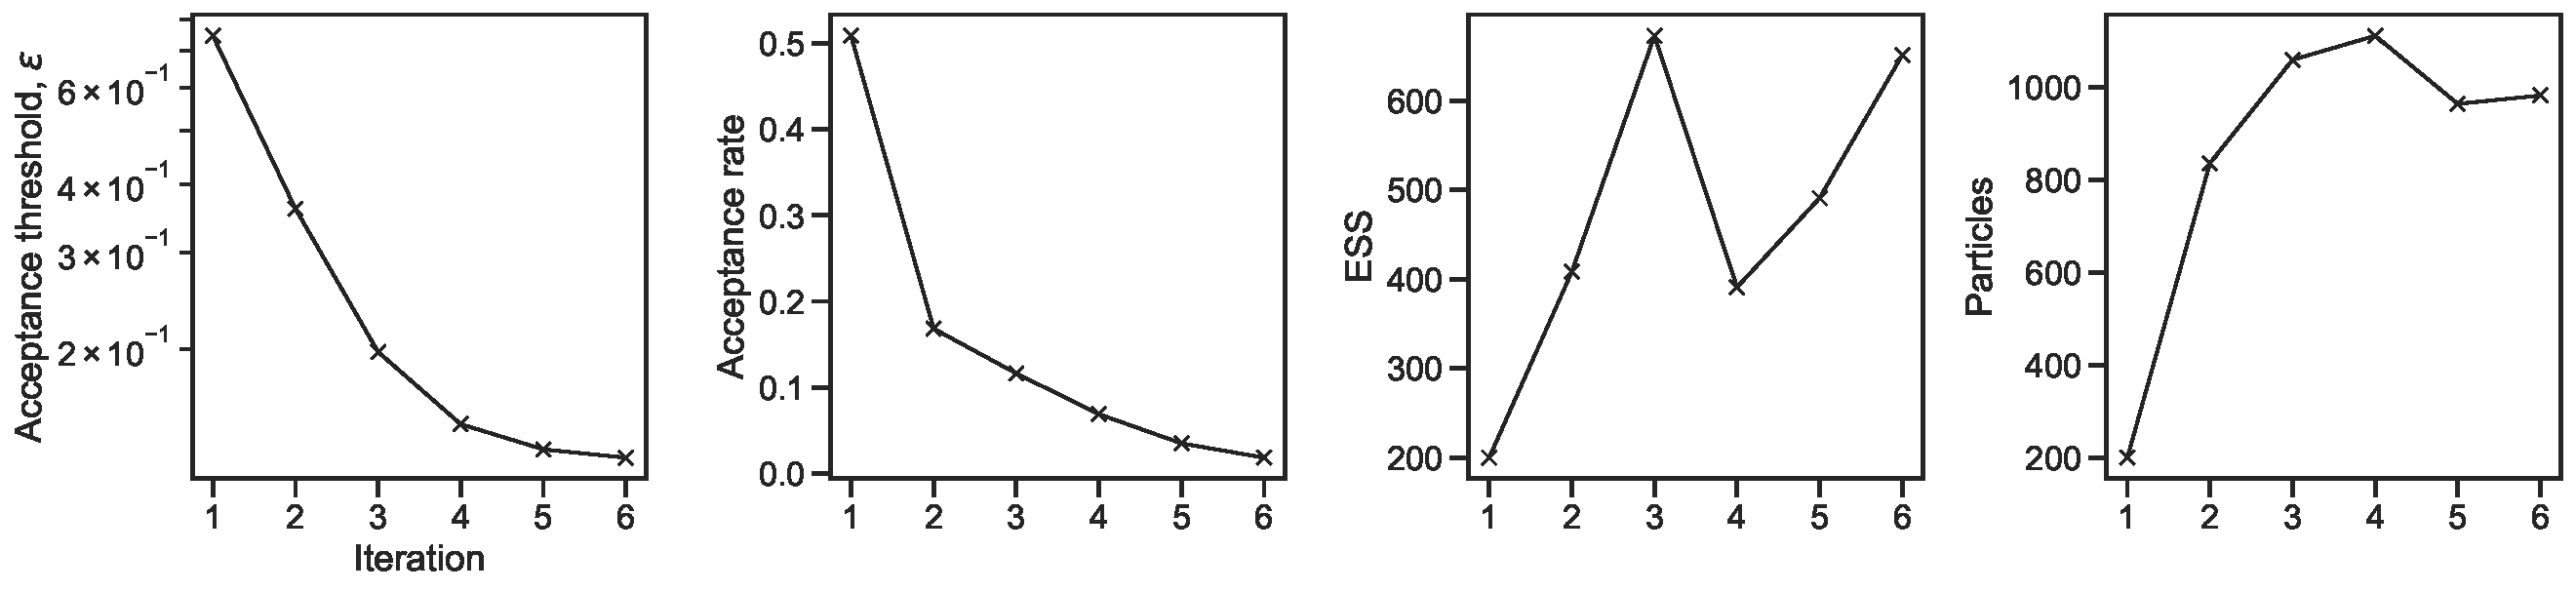
\includegraphics[width=\textwidth]{../figures/ess.pdf}
     \label{fig:convergence-B}
  \end{subfigure}
    \caption{
    \textbf{Single-locus model inference convergence.} 
    The ABC-SMC algorithm was used to infer the parameters of the single-locus model. \textbf{(A-E)} The approximate posterior distributions of model parameters at each iteration of the ABC-SMC algorithm demonstrates convergence, as the posterior did not significantly change after the first iteration, $t=1$.
    \textbf{(F-I)} ABC-SMC measures of convergence. After iteration number 6, the acceptance threshold was $\epsilon=0.13$, the acceptance rate was $0.018$, the number of particles was 982, and the effective sample size ESS=651.
}
    \label{fig:convergence}
\end{figure}


% Fig Validation of posteriors
%% generated with diff-runs.ipynb
\begin{figure}[h]
    \centering
      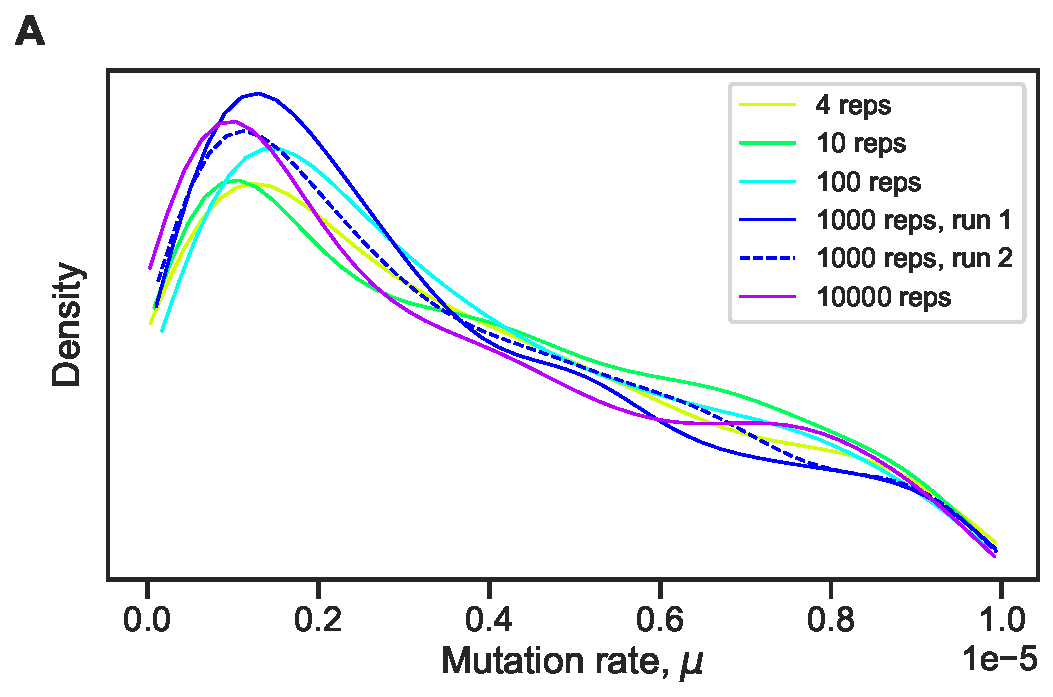
\includegraphics[width=0.45\textwidth]{../figures/runs-A.pdf}      
      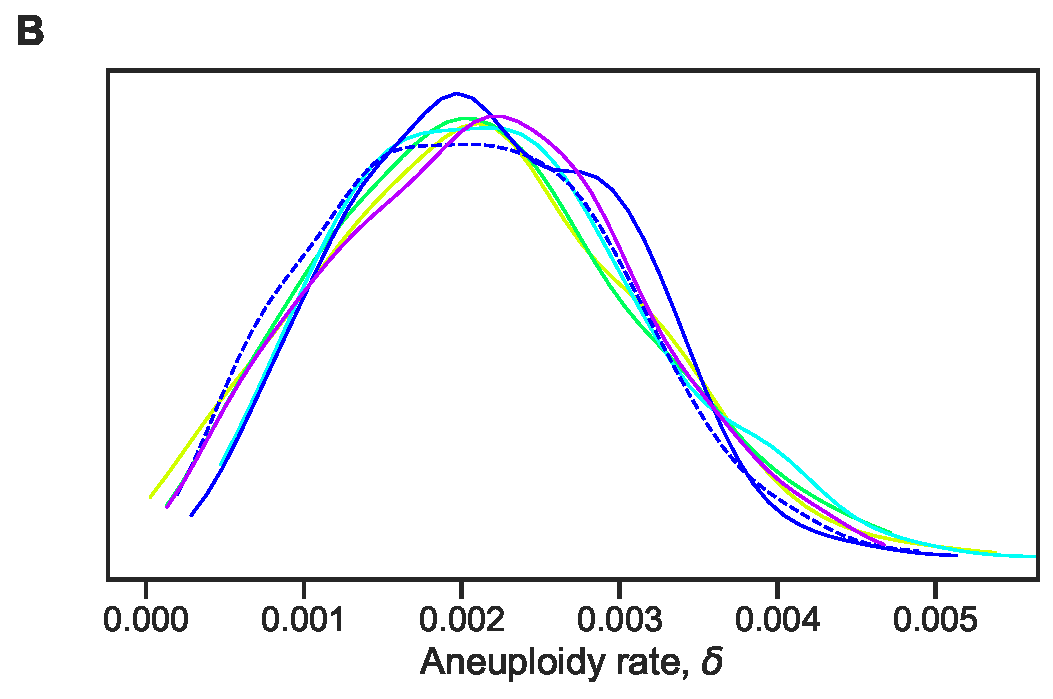
\includegraphics[width=0.45\textwidth]{../figures/runs-B.pdf}    
      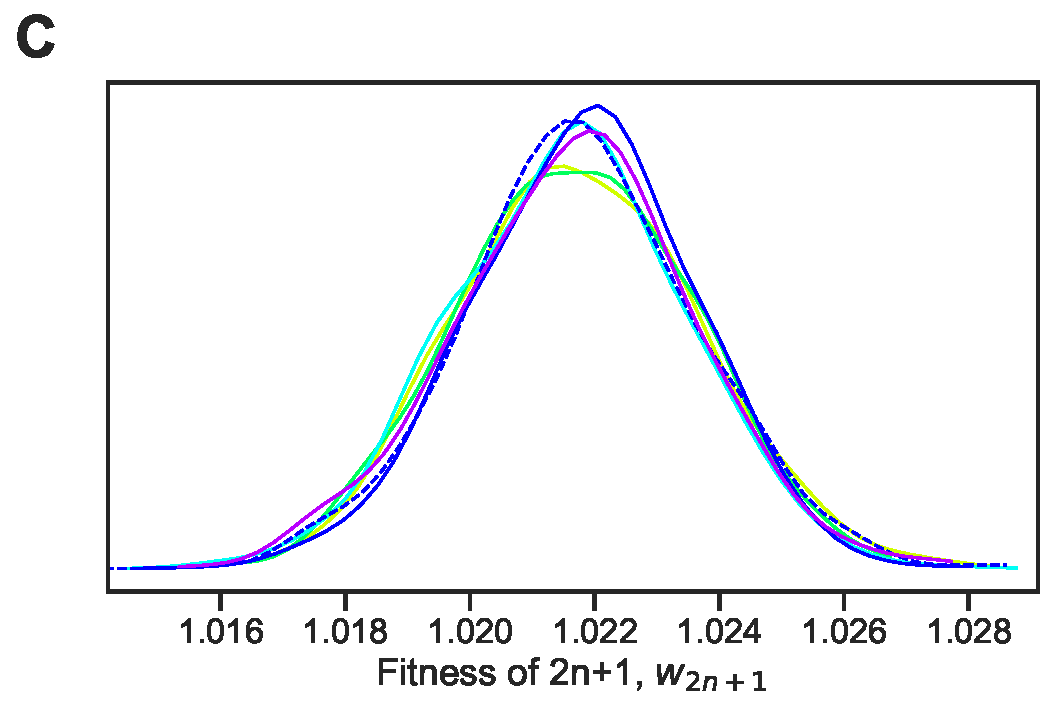
\includegraphics[width=0.325\textwidth]{../figures/runs-C.pdf}      
      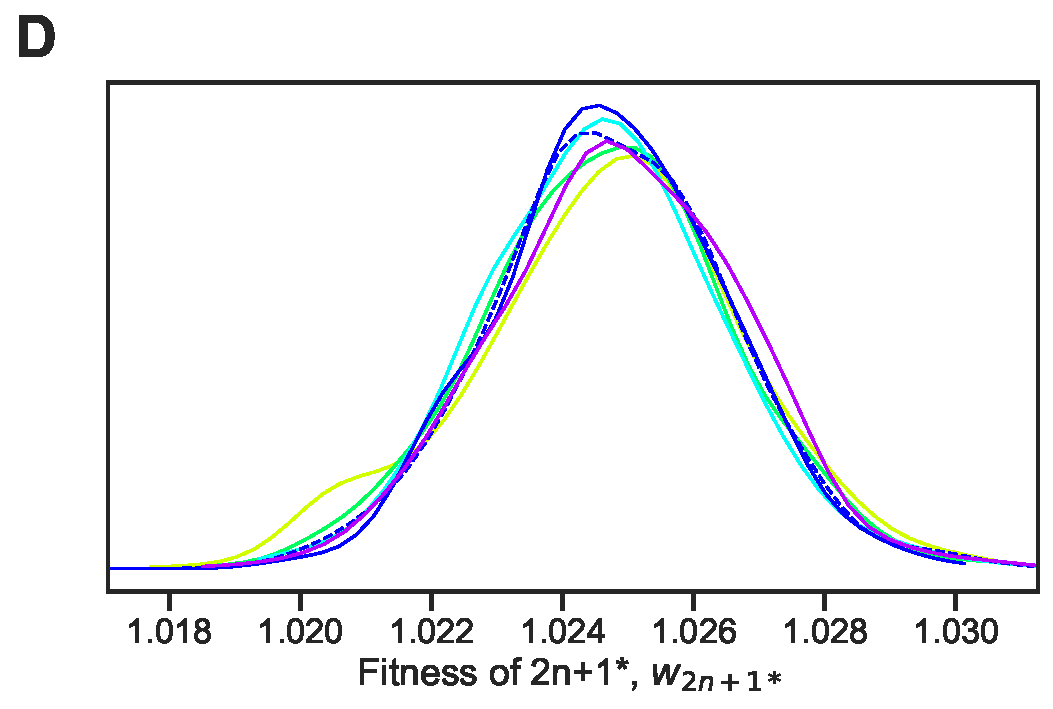
\includegraphics[width=0.325\textwidth]{../figures/runs-D.pdf}      
      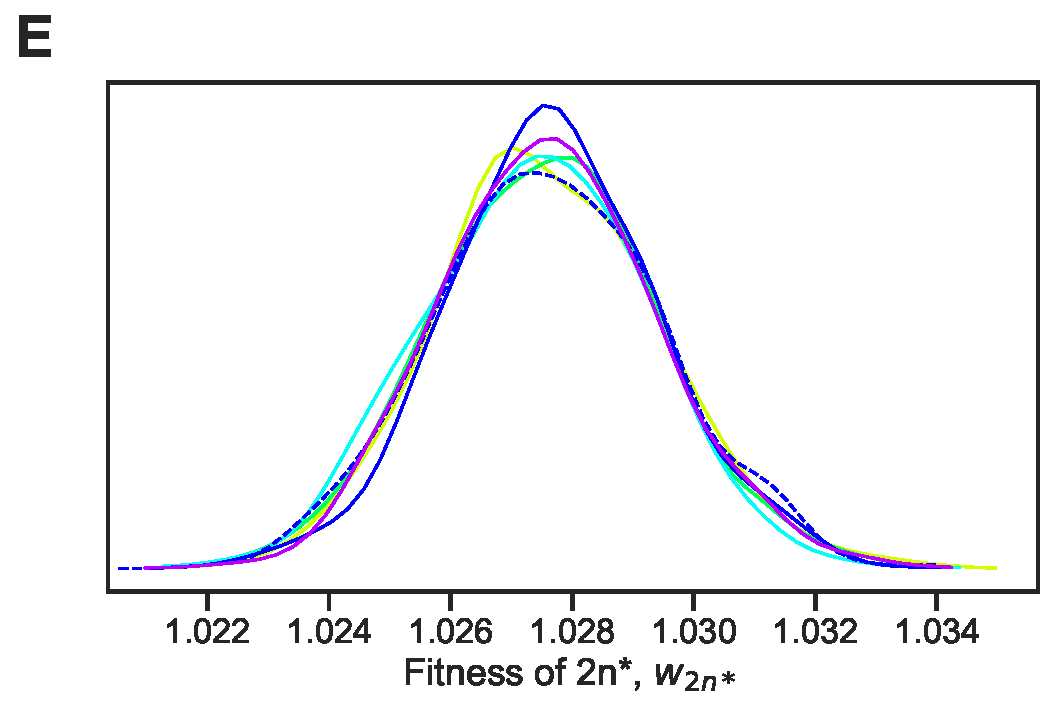
\includegraphics[width=0.325\textwidth]{../figures/runs-E.pdf} 
       \caption{
    \textbf{Posterior distribution validation.}
    The posterior distribution of the single-locus model parameters is roughly the same regardless of the number of simulations (4-10,000 replicates) used to approximate the likelihood (\autoref{eq:heatstress-likelihood}).
    % TODO add "Density" to y label in C
    } 
     
     \label{fig:seeds}
 \end{figure}

\end{document}  